\documentclass[letterpaper]{jpconf}

\usepackage{amsfonts}
\usepackage{amsmath}
\usepackage{amssymb}
\usepackage{amsthm}
\usepackage{graphicx}
\usepackage{hyperref}
\hypersetup{
  bookmarksnumbered = true,
  bookmarksopen=false,
  pdfborder=0 0 0,         % make all links invisible, so the pdf looks good when printed
  pdffitwindow=true,      % window fit to page when opened
  pdfnewwindow=true, % links in new window
  colorlinks=true,           % false: boxed links; true: colored links
  linkcolor=blue,            % color of internal links
  citecolor=magenta,    % color of links to bibliography
  filecolor=magenta,     % color of file links
  urlcolor=cyan              % color of external links
}

\newcommand{\deriv}[2]{\frac{d #1}{d #2}}
\newcommand{\pderiv}[2]{\frac{\partial #1}{\partial #2}}
\newcommand{\vect}[1]{\boldsymbol{#1}}
\newcommand{\f}[2]{\frac{#1}{#2}}
\newcommand{\dx}{\Delta x}
\newcommand{\pd}[2]{\partial_{#2}{#1}}
\newcommand{\bx}{\vect{x}}
\newcommand{\bK}{\vect{K}}
\newcommand{\cT}{\mathcal{T}}
\newcommand{\xL}{x_{\textnormal{\tiny\textsc{L}}}}
\newcommand{\xH}{x_{\textnormal{\tiny\textsc{H}}}}
\newcommand{\xMin}{x_{\textnormal{\tiny m}}}
\newcommand{\xMax}{x_{\textnormal{\tiny M}}}
\newcommand{\trans}{\textnormal{\tiny\textsc{T}}}
\newcommand{\leftState}{\textnormal{\tiny\textsc{L}}}
\newcommand{\rightState}{\textnormal{\tiny\textsc{R}}}
\newcommand{\TCI}{\textnormal{\tiny\textsc{TCI}}}
\newcommand{\shock}{\textnormal{\tiny\textsc{Sh}}}
\newcommand{\thornado}{\texttt{thornado}}

\newcommand{\ee}[1]{{\color{red} EE:~#1}}

\begin{document}
\title{\thornado-hydro: towards discontinuous galerkin methods for supernova hydrodynamics}

\author{Eirik Endeve}
\address{Computational \& Applied Mathematics, Oak Ridge National Laboratory, Oak Ridge, TN 37831 USA}
\address{Department of Physics and Astronomy, University of Tennessee Knoxville, TN 37996-1200}
\ead{endevee@ornl.gov}

\author{Kristopher Andrew, Brandon Barker, Jesse Buffaloe, Samuel Dunham, David Pochik, Juliana Pulsinelli, Nick Roberts}

\begin{abstract}
The toolkit for high-order neutrino-radiation hydrodynamics (\thornado) is being developed for simulations of core-collapse supernovae (CCSN) and related problems.  
Current capabilities in \thornado\ include solvers for the Euler equations --- in non-relativistic and special relativistic limits --- and the two-moment model of neutrino transport.  
The spatial discretization in \thornado\ is based on the discontinuous Galerkin (DG) method, which is receiving increased attention from the computational astrophysics community.  
In this paper, we provide an overview of the numerical methods for the Euler equations in \thornado, and present some encouraging preliminary numerical results from a set of basic tests in one and two spatial dimensions.  
\end{abstract}

\section{Introduction}

\ee{Introduction coming soon.}

\section{Discontinuous Galerkin Method}

Excellent books and review articles on the DG method are available (see, e.g., \cite{cockburnShu_1998,cockburnShu_2001,hesthavenWarburton_2008,shu_2016} and references therein), and we will not go into too much detail here.  
However, we review some key concepts to introduce notation, and emphasize specific choices in our implementation in \thornado.  
To this end, we consider a system of conservation laws with sources of the form
\begin{equation}
  \pd{}{t}\big(\,\sqrt{\gamma}\,\vect{U}\,\big)
  +\pd{}{i}\Big(\,\sqrt{\gamma}\,\vect{F}^{i}(\vect{U})\,\Big)
  =\sqrt{\gamma}\,\vect{S}(\vect{U}),
  \label{eq:extendedEulerCompact}
\end{equation}
where $\vect{U}$ is the evolved state vector, $\vect{F}^{i}$ the fluxes, and $\vect{S}$ the source vector.  
We use a formulation of the equations sufficiently general to accommodate curvilinear spatial coordinates encoded in the metric $\gamma_{ij}$, giving the squared line element $ds^{2}=\gamma_{ij}dx^{i}dx^{j}$, whose determinant is $\gamma$.  
To solve Eq.~\eqref{eq:extendedEulerCompact}, the computational domain $D$ is divided into a disjoint union $\cT$ of open elements $\bK$, so that $D = \cup_{\bK \in \cT}\bK$.  
We require that each element is a box in the logical coordinates; i.e.,
\begin{equation}
  \bK=\{\vect{x} : x^{i} \in K^{i} := (\xL^{i},\xH^{i})\}, 
\end{equation}
with the surface elements denoted $\partial\bK^{i}=\times_{j\ne i}K^{j}$.  
We let $V_{\bK}$ denote the proper element volume
\begin{equation}
  V_{\bK} = \int_{\bK}dV, \quad\text{where}\quad dV = \sqrt{\gamma}\,\prod_{i=1}^{d}dx^{i}.  
\end{equation}
We also define as a set $\bx=\{\tilde{\bx}^{i},x^{i}\}$, and $\dx^{i}=\xH^{i}-\xL^{i}$.  

We let the approximation space for the DG method, $\mathbb{V}^{k}$, be constructed from the tensor product of one-dimensional polynomials of maximal degree $k$.  
(Functions in $\mathbb{V}^{k}$ can be discontinuous across element interfaces.)  
The semi-discrete DG problem is to find $\vect{U}_{h}\in\mathbb{V}^{k}$ (which approximates $\vect{U}$ in Eq.~\eqref{eq:extendedEulerCompact}) such that for all $v\in\mathbb{V}^{k}$ and all $\bK\in\mathcal{T}$
\begin{align}
  &\partial_{t}\int_{\bK}\vect{U}_{h}\,v\,dV
  +\sum_{i=1}^{d}\int_{\partial\bK^{i}}\big(\,\sqrt{\gamma}\,\widehat{\vect{F}}^{i}(\vect{U}_{h})\,v\big|_{\xH^{i}}-\sqrt{\gamma}\,\widehat{\vect{F}}^{i}(\vect{U}_{h})\,v\big|_{\xL^{i}}\,\big)\,d\tilde{\bx}^{i} \nonumber \\
  &\hspace{24pt}
  -\sum_{i=1}^{d}\int_{\bK}\vect{F}^{i}(\vect{U}_{h})\,\pd{v}{i}\,dV
  =\int_{\bK}\vect{S}(\vect{U}_{h})\,v\,dV.  
  \label{eq:semidiscreteDG}
\end{align}
In Eq.~\eqref{eq:semidiscreteDG}, $\widehat{\vect{F}}^{i}(\vect{U}_{h})$ is a numerical flux approximating the flux on the $i$th surface of $\bK$.  
The numerical flux function $\vect{f}^{i}$ evaluates the numerical flux given values from both sides of an element interface; i.e.,
\begin{equation}
  \widehat{\vect{F}}^{i}(\vect{U}_{h})=\vect{f}^{i}(\vect{U}_{h}(x^{i,-},\tilde{\bx}^{i}),\vect{U}_{h}(x^{i,+},\tilde{\bx}^{i})),
\end{equation}
where superscripts $-/+$, e.g., in the arguments of $\vect{U}_{h}$, indicate that the function is evaluated to the immediate left/right of $x^{i}$.  
We use the Harten-Lax-van Leer (HLL) flux \cite{harten_etal_1983} or the HLLC flux \cite{toro_etal_1994,mignoneBodo_2005} for all the numerical experiments presented in Section~\ref{sec:numerical}.  

We provide further details on the DG method to arrive at the equations that are actually evolved in \thornado.  
We start by introducing some notation, defining the polynomial expansion for $\vect{U}_{h}$, and the quadrature rules used to evaluate the integrals in Equation~\eqref{eq:semidiscreteDG}.  
Then we provide explicit expressions for each of the terms in Equation~\eqref{eq:semidiscreteDG}.  
For simplicity we consider one spatial dimension ($d=1$) and drop indices denoting the spatial dimension.  
In each element $K$, we use a nodal representation of the conserved variables $\vect{U}$; i.e.,
\begin{equation}
  \vect{U}(x,t)\approx
  \vect{U}_{h}(x,t)=\sum_{i=1}^{N}\vect{U}_{i}(t)\,\ell_{i}(x),
  \label{eq:conservedNodalExpansion}
\end{equation}
where $\ell_{i}(x)$ are Lagrange polynomials
\begin{equation}
  \ell_{i}(\eta)=
  \prod_{\substack{j=1\\j\ne i}}^{N}\f{\eta-\eta_{j}}{\eta_{i}-\eta_{j}},
\end{equation}
defined on the reference element $I = \{ \eta : \eta \in (-0.5,0.5) \}$, and constructed to interpolate the node set $S_{N}=\{\eta_{i}\}_{i=1}^{N}\subset I$.  
The spatial coordinate $x$ and the reference coordinate $\eta$ are related by the mapping $x(\eta)=\xL+(0.5+\eta)\,\dx$.  
Then, for any $\eta_{j}\in S_{N}$, $\ell_{i}(\eta_{j})=\delta_{ij}$, so that $\vect{U}_{h}(x(\eta_{j}),t)=\vect{U}_{j}(t)$.  
We introduce numerical quadratures to evaluate the integrals in Equation~\eqref{eq:semidiscreteDG}.  
First we define the $M$-point quadrature $Q_{M}:C^{0}(I)\to\mathbb{R}$ with abscissas $\hat{S}_{M}=\{\eta_{q}\}_{q=1}^{M}$ and weights $\{w_{q}\}_{q=1}^{M}$, normalized such that $\sum_{q=1}^{M}w_{q}=1$.  
The $M$-point Legendre-Gauss quadrature, which we use, integrates polynomials of degree $\le 2M-1$ exactly.  
Then, if $P(x)$ is such a polynomial, we have
\begin{equation}
  \f{1}{\dx}\int_{K}P(x)\,dx=\int_{I}P(\eta)\,d\eta=Q_{N}\big[P\big]\equiv\sum_{q=1}^{M}w_{q}\,P(\eta_{q}).  
\end{equation}

Note that the interpolation points $S_{N}$ and the quadrature points $\hat{S}_{M}$ generally do not coincide.  
However, for sake of computational efficiency we let $M=N$ and $S_{N}=\hat{S}_{N}$, which is a spectral-type nodal collocation DG approximation \cite{bassi_etal_2013}.  
Inserting Eq.~\eqref{eq:conservedNodalExpansion} into Eq.~\eqref{eq:semidiscreteDG}, letting $v(x)=\ell_{k}(x)$, and using the quadratures defined above, we obtain
\begin{align}
  \pd{}{t}\int_{K}\vect{U}_{h}\,v\,dV
  &\approx w_{k}\,\sqrt{\gamma}_{k}\,\pd{}{t}\vect{U}_{k}\,\dx
  \label{eq:timeDerivativeTerm}
\end{align}
for the time derivative term.  
The integration is approximate since we use the Legendre-Gauss quadrature rule with the nodal points given by the expansion in Eq.~\eqref{eq:conservedNodalExpansion}.  
Since $\ell_{i}(\eta_{k})=\delta_{ik}$, this leads to a diagonal mass matrix, and simplifies the implementation.  
Similarly, we obtain
\begin{align}
  \int_{K}\vect{S}(\vect{U}_{h})\,v\,dV
  &\approx w_{k}\,\sqrt{\gamma}_{k}\,\vect{S}(\vect{U}_{k})\,\dx.
  \label{eq:sourceTerm}
\end{align}
for the source term.  
Finally, the volume term (last term on the left-hand side of Eq.~\eqref{eq:semidiscreteDG}) becomes
\begin{equation}
  \int_{K}\vect{F}(\vect{U}_{h})\,\pderiv{v}{x}\,dV
  \approx \sum_{q=1}^{N}w_{q}\,\sqrt{\gamma}_{q}\,\vect{F}(\vect{U}_{q})\,\pderiv{\ell_{k}}{\eta}(\eta_{q}).
  \label{eq:volumeTerm}
\end{equation}
Using Eqs.~\eqref{eq:timeDerivativeTerm}-\eqref{eq:volumeTerm} in Eq.~\eqref{eq:semidiscreteDG} results in the semi-discrete form
\begin{align}
  \deriv{\vect{U}_{k}}{t}
  =-\f{1}{w_{k}\sqrt{\gamma}_{k}\dx}
  \Big\{
  \Big[\,
    \sqrt{\gamma}\widehat{\vect{F}}\ell_{k}\big|_{\xH}
    -\sqrt{\gamma}\widehat{\vect{F}}\ell_{k}\big|_{\xL}
  \,\Big]
  -\sum_{q=1}^{N}w_{q}\,\sqrt{\gamma}_{q}\,\vect{F}(\vect{U}_{q})\,\pderiv{\ell_{k}}{\eta}(\eta_{q})
  \Big\} + \vect{S}(\vect{U}_{k}).
  \label{eq:semidiscreteDiscretized}
\end{align}
Eq.~\eqref{eq:semidiscreteDiscretized} comprises a system of ordinary differential equations (ODEs), which are integrated in time with an ODE solver.  
In section~\ref{sec:numerical} we use the optimal third-order strong stability-preserving Runge-Kutta (SSP-RK3) method from \cite{shuOsher_1988}.  

Limiting of the polynomial representation $\vect{U}_{h}$, to reduce oscillations and prevent non-physical states, is a critical step in the DG algorithm.  
We use the TVD-type slope limiter based on limiting characteristic variables discussed in \cite{cockburnShu_1998}.  
To prevent excessive limiting (e.g., at smooth extrema), we use the troubled-cell indicator (TCI) of \cite{fuShu_2017}.  
\begin{equation}
  I_{\bK}(G) = \f{\sum_{j}|G_{\bK}-G_{\bK}^{(j)}|}{\max_{j}|G_{\bK^{(j)}}^{(j)}|},
  \label{eq:indicator}
\end{equation}
where $G\in\vect{G}\subseteq\vect{U}$.  
(Here, $\vect{G}$ consists of the first and last element of $\vect{U}$.)  
In Eq.~\eqref{eq:indicator}, the sum in the numerator and the $\max$ in the denominator extend over the neighboring elements sharing face with the target element $\bK$.  
$G_{\bK}$ is the cell average in $\bK$, $G_{\bK}^{(j)}$ is the cell average computed by extrapolating the polynomial representation from the neighbor element $\bK^{(j)}$ into $\bK$, and $G_{\bK^{(j)}}^{(j)}$ is the cell average native to $\bK^{(j)}$.  
An element is flagged for limiting if $I_{\bK}(G)>C_{\TCI}$ for any $G\in\vect{G}$.  
To prevent negative mass density and pressure (and superluminal velocity for the relativistic Euler equations), we follow the approaches in \cite{zhangShu_2010,wuTang_2015,qin_etal_2016}.  

\section{Preliminary Numerical Results}
\label{sec:numerical}

In this section we show preliminary numerical results obtained with the DG method implemented in \thornado\ to solve the non-relativistic and special relativistic Euler equations.  
We use the ideal gas equation of state where the pressure $p$ is related to the internal energy density $e$ by $p=(\Gamma-1)e$, and where $\Gamma$ is the (constant) adiabatic index.  
Let the $d$-dimensional computational domain be $D=\times_{i=1}^{d}[\xMin^{i},\xMax^{i}]$, where $\xMin^{i}$ and $\xMax^{i}$ denote the coordinates of the inner and outer boundary in the $i$-th coordinate direction, respectively.  
We use polynomials of degree $k=2$ combined with SSP-RK3 time stepping, and all the tests were run with a Courant-Friedrichs-Lewy (CFL) factor of $C=0.1$.  
We use the HLL Riemann solver when solving the non-relativistic Euler equations and the HLLC Riemann solver when solving the special relativistic Euler equations.  
The purpose of the tests is gauge the performance of the DG implementation on a set of benchmarks as an initial measure of its suitability for future for CCSN simulations.  

\subsection{Non-relativistic (NR) hydrodynamics}

For the NR Euler equations, the state, flux, and source vectors in Eq.~\eqref{eq:extendedEulerCompact} are
\begin{equation}
  \vect{U}=\big(\rho,\rho u_{j},E\big)^{\trans},~
  \vect{F}^{i}=\big(\rho\,u^{i},\Pi^{i}_{~j},(E+p)u^{i}\big)^{\trans},~
  \text{and}~
  \vect{S}=\big(0,\f{1}{2}\Pi^{ik}\pd{\gamma_{ik}}{j}-\rho\pd{\Phi}{j},-\rho u^{i}\pd{\Phi}{i}\big)^{\trans},
\end{equation}
where $\rho$ and $u^{i}$ are the mass density and components of the fluid three-velocity, respectively.  
The stress tensor is $\Pi^{i}_{~j}=\rho u^{i} u_{j}+p\delta^{i}_{~j}$, and $E=e+\f{1}{2}\rho u_{i} u^{i}$ is the fluid (internal plus kinetic) energy density.  
The sources are due to curvilinear coordinates and Newtonian gravity.  

\subsubsection{Sod Shock Tube}

The first test is the classical Riemann problem due to Sod \cite{sod_1978}, computed using Cartesian coordinates.  
The one-dimensional computational domain is $D=[0,1]$, and a discontinuity is initially located at $x^{1}=0.5$, separating the left and right states
\begin{equation*}
  \vect{U}_{\leftState}=(1.0,\vect{0.0},2.5)^{\trans}\quad\text{and}\quad
  \vect{U}_{\rightState}=(0.125,\vect{0.0},0.25)^{\trans},
\end{equation*}
where the adiabatic index is $\Gamma=1.4$.  
The test is run with $100$ elements until $t=0.2$, using $C_{\TCI}=0.03$.  
Results are plotted in the left panel of Figure~\ref{fig:SodSedov}.  
The DG method captures the main features of the solution well without introducing noticeable oscillations near the discontinuities.  
\begin{figure}[h]
  \centering
  \begin{minipage}{18pc}
    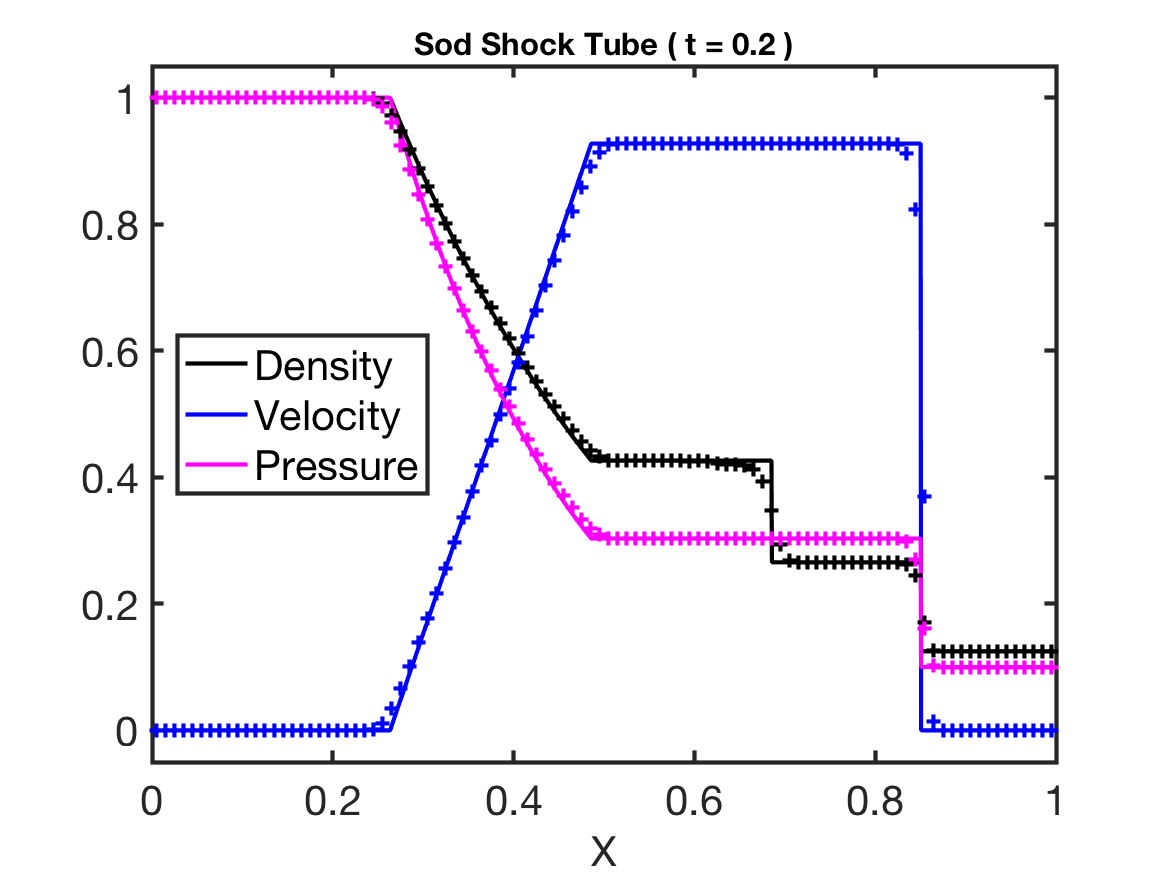
\includegraphics[width=18pc]{./Figures/Sod_Astronum_2018}
  \end{minipage}\hspace{0.5pc}%
  \begin{minipage}{18pc}
    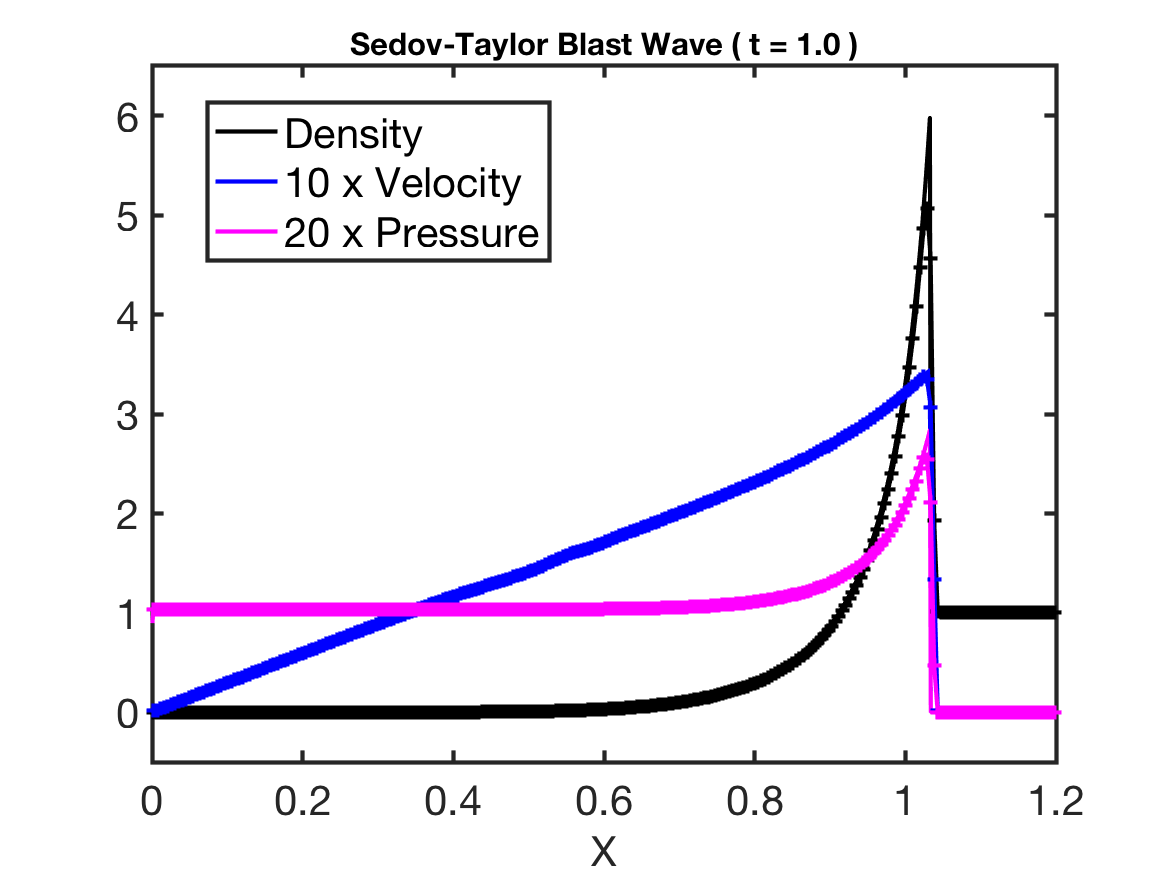
\includegraphics[width=18pc]{./Figures/Sedov_Astronum_2018}
  \end{minipage}
  \caption{\label{fig:SodSedov}{\it Left panel:} numerical solution of Sod's problem using $100$ elements (plusses) compared with the exact solution (solid lines; from \cite{toro_1999}).  {\it Right panel:} numerical solution of the Sedov-Taylor blast wave using $256$ elements (plusses) against the exact solution (solid lines).}
\end{figure}

\subsubsection{Sedov-Taylor Blast Wave}

This test, detailed in \cite{sedov_1959} (see also {\S}99 in \cite{landauLifshitz_1979}), is computed in spherical polar coordinates with the assumption of spherical symmetry.\footnote{In this paper, all tests in spherical polar coordinates are computed with the assumption of spherical symmetry.}
The computational domain is $D=[0,1.2]$, and the initial condition consists of a fluid at rest with density $\rho=1$.  
The adiabatic index is $\Gamma=1.4$, and an amount of thermal energy equal to $1$ is released in the innermost element.  
We use $256$ elements and run until $t=1$, using $C_{\TCI}=0.03$.  
Again, the DG method captures the characteristic of the exact solution well.  
The maximum density in the shock is somewhat lower for the numerical solution than the exact value (about $5$ versus $6$).  

\subsubsection{Shu-Osher Shock Tube}

This test from \cite{shuOsher_1989} is suitable for measuring the amount of dissipation in a numerical scheme.  
The one-dimensional computational domain is $D=[-5,5]$, and a discontinuity is placed at $x^{1}=-4$, separating the states
\begin{equation*}
  \vect{U}_{\leftState}=\big( 3.857143, 10.14185, 0.0, 0.0, 39.16667 \big)^{\trans}\quad\text{and}\quad
  \vect{U}_{\rightState}=\big( 1+0.2\times\sin(5 x^{1}), \vect{0.0}, 2.5 \big)^{\trans},
\end{equation*}
where the adiabatic index is $\Gamma=1.4$.  
The density variations ahead of the Mach=3 shock are compressed through the shock and result in higher-frequency variations downstream, which can be difficult to capture with an excessively dissipative scheme.  

We have run this test with $200$ elements to $t=1.8$.  
In the two upper panels of Figure~\ref{fig:ShuOsher} we plot the density for various values of the troubled-cell indicator threshold $C_{\TCI}$; $0.0$ (full limiting, green), $0.03$ (magenta), $0.3$ (red), and $3.0$ (blue).  
(Larger values of $C_{\TCI}$ imply less limiting.)  
The results are compared with a reference solution computed with $2048$ elements.  
With full limiting, the scheme is not able to capture the density variations behind the shock (cf. upper right panel in Figure~\ref{fig:ShuOsher}).  
When $C_{\TCI}=0.03$, the variations are resolved, but the amplitudes are significantly reduced when compared with the reference solution.  
With $C_{\TCI}=3.0$, the variations are well resolved, and the amplitudes are comparable to the reference.  
\begin{figure}[h]
  \centering
  \begin{minipage}{18pc}
    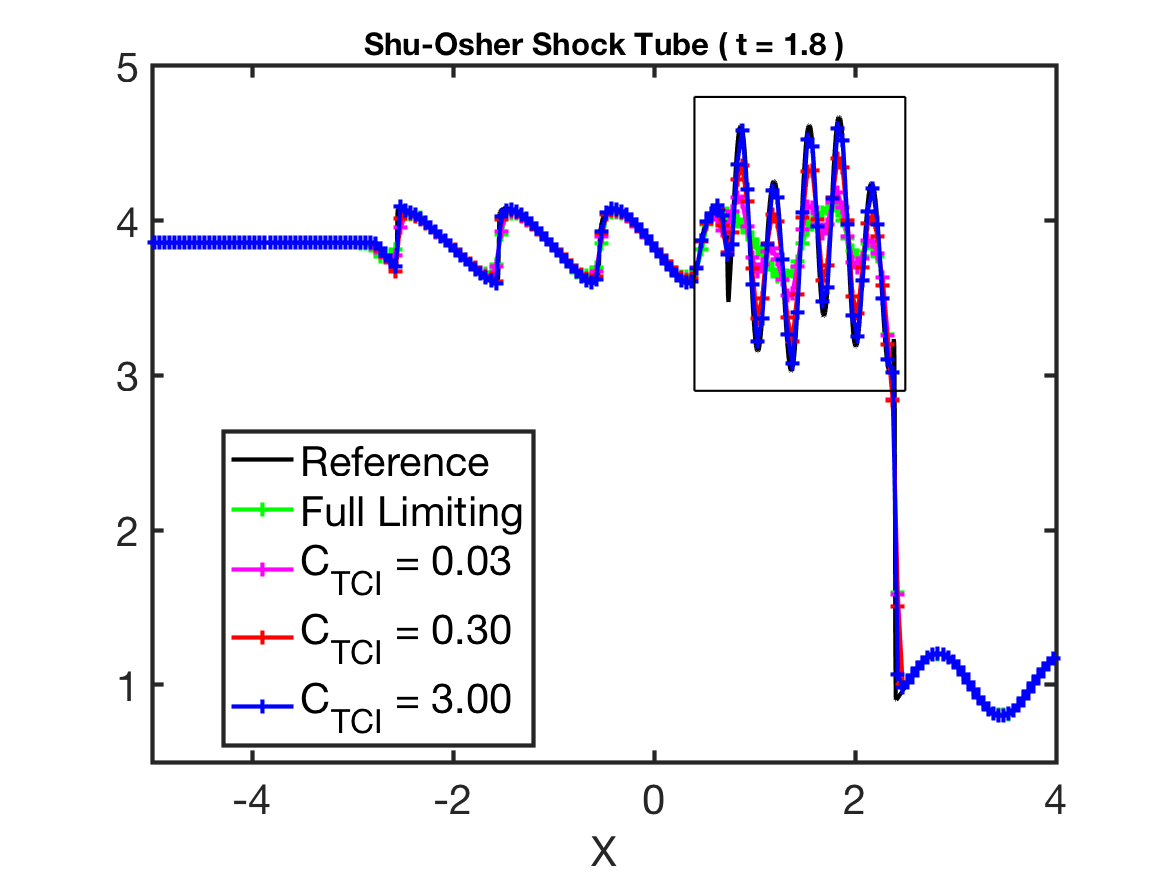
\includegraphics[width=18pc]{./Figures/ShuOsher_Astronum_2018}
  \end{minipage}\hspace{0.5pc}%
  \begin{minipage}{18pc}
    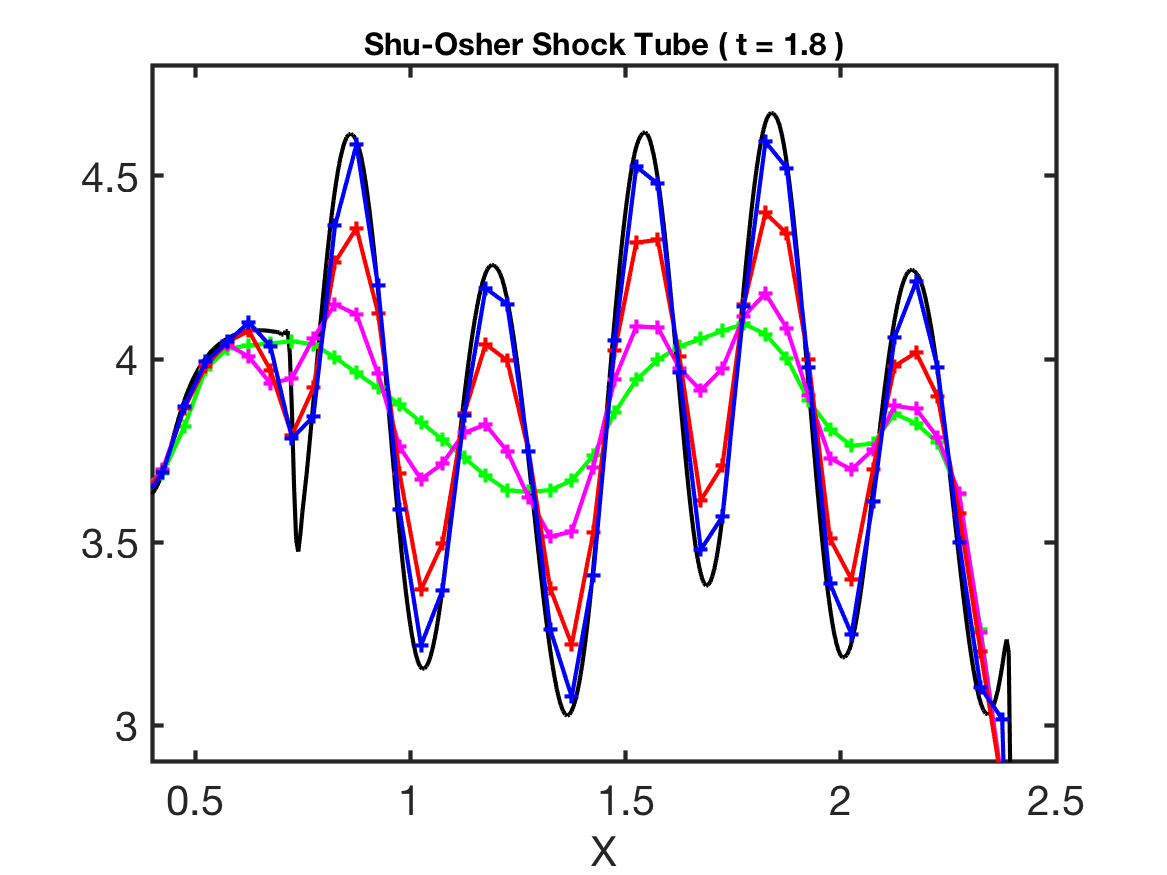
\includegraphics[width=18pc]{./Figures/ShuOsher_Inset_Astronum_2018}
  \end{minipage} \\
  \begin{minipage}{12pc}
    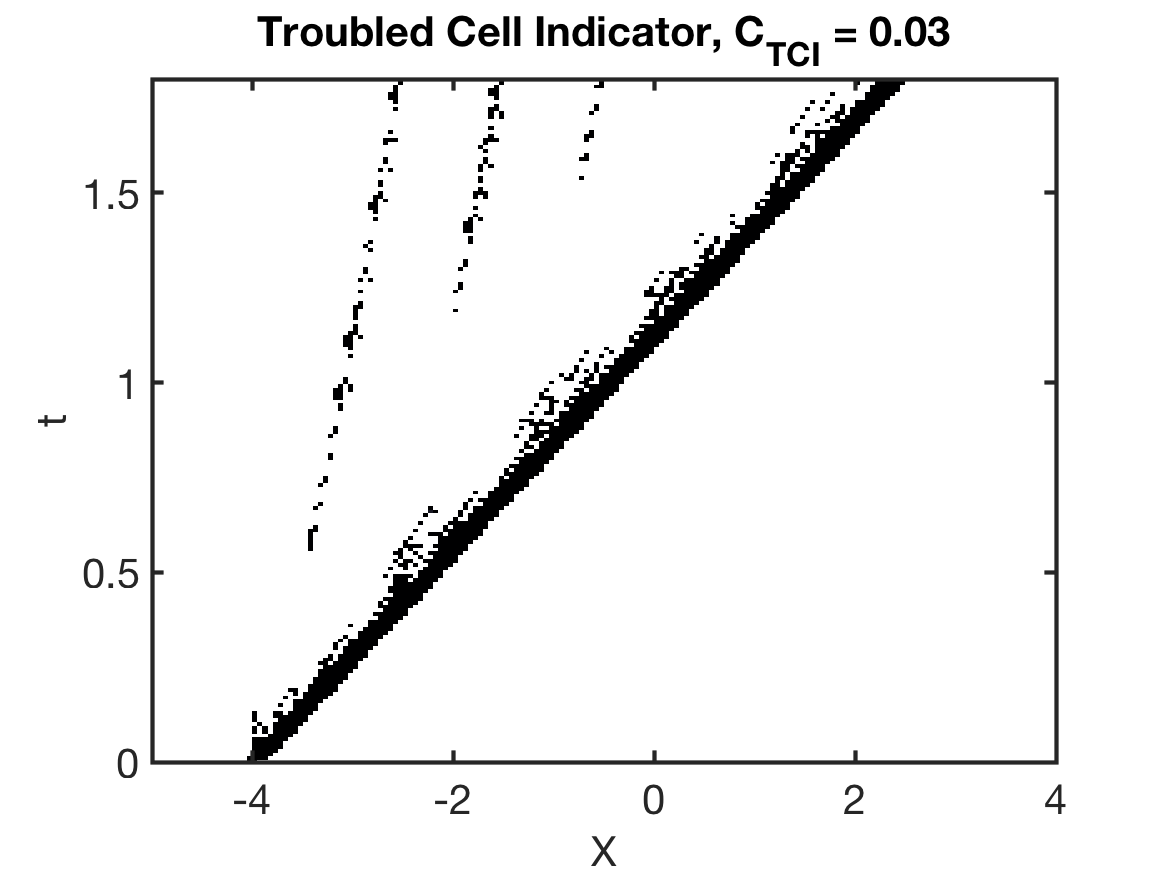
\includegraphics[width=12pc]{./Figures/ShuOsher_TCI_0015_Astronum_2018}
  \end{minipage}\hspace{0.5pc}%
  \begin{minipage}{12pc}
    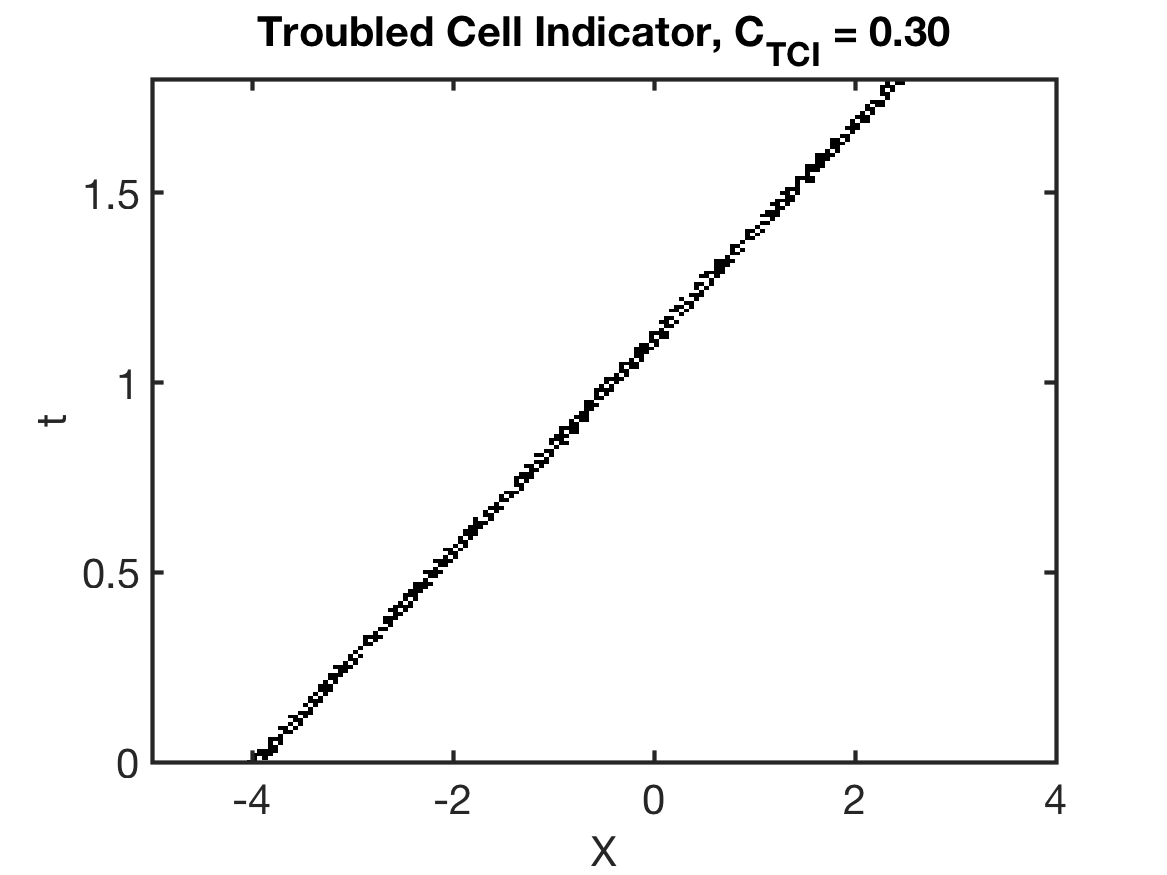
\includegraphics[width=12pc]{./Figures/ShuOsher_TCI_0150_Astronum_2018}
  \end{minipage}\hspace{0.5pc}
  \begin{minipage}{12pc}
    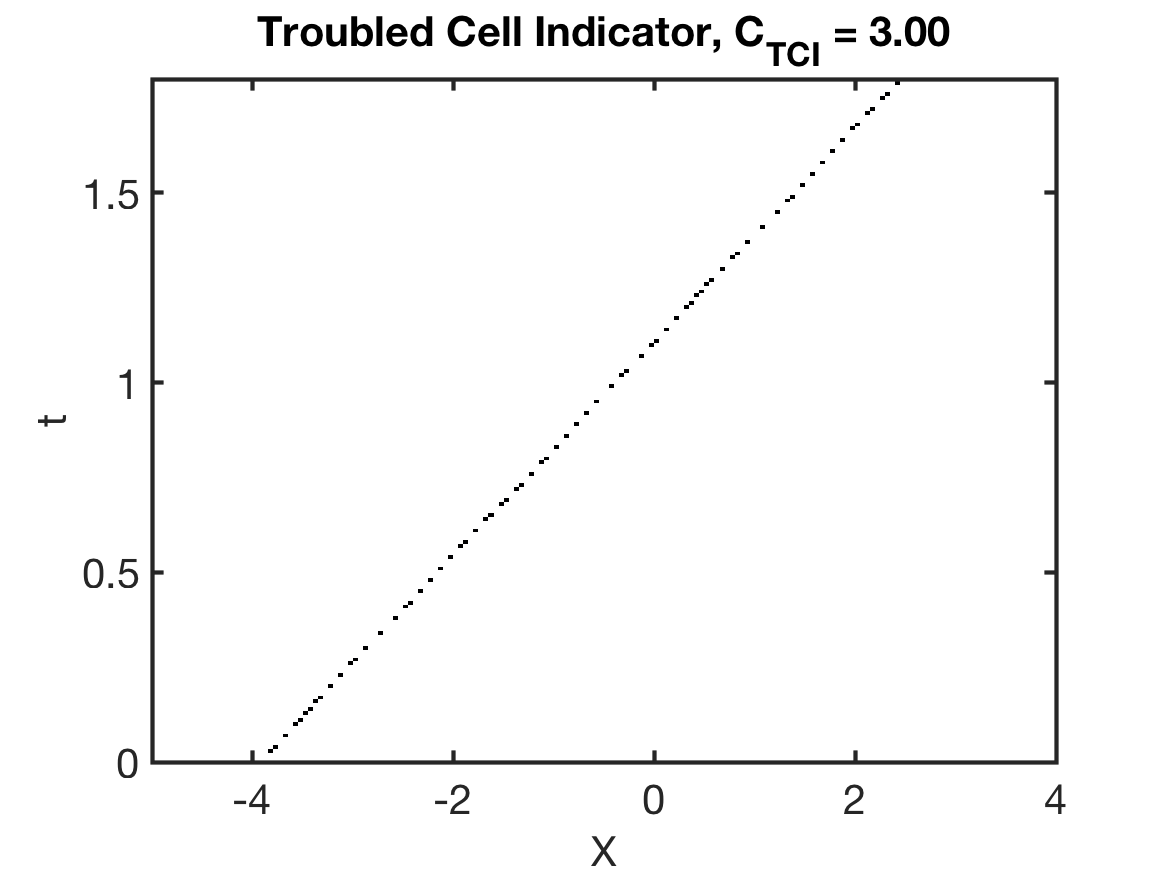
\includegraphics[width=12pc]{./Figures/ShuOsher_TCI_1500_Astronum_2018}
  \end{minipage}
  \caption{\label{fig:ShuOsher}Results for the Shu-Osher shock tube problem computed with $200$ elements.  The upper panels show the mass density at $t=1.8$ for various values of the troubled-cell indicator threshold $C_{\TCI}$, compared with a high-resolution (2048 elements) reference solution.  In the lower panels we show elements flagged for limiting in the $xt$-plane for various values of $C_{\TCI}$.}
\end{figure}
In the lower panels of Figure~\ref{fig:ShuOsher} we plot locations in the $xt$-plane where elements have been flagged for limiting by the troubled-cell indicator: $C_{\TCI}=0.03$ (left), $C_{\TCI}=0.3$ (middle), and $C_{\TCI}=3.0$ (right).  
With $C_{\TCI}=0.03$, limiting is triggered in a wide region around the shock and also around the peaks of the three leftmost density variations seen in upper left panel in Figure~\ref{fig:ShuOsher}.  
With $C_{\TCI}=3.0$, limiting is only triggered in the shock.  

\subsubsection{Kelvin-Helmholtz (KH) Instability}
This hydrodynamic instability is of significant astrophysical relevance --- including in the explosion phase of CCSNe.  
It may occur in the interface separating fluids in relative motion.  
We compute this problem on the unit square $D=[0,1]\times[0,1]$, imposing periodic boundary conditions, and with initial conditions and single-mode perturbation taken from \cite{mcnally_etal_2012}.  
We use $256^{2}$ elements and evolve until $t=3.0$, well into the nonlinear regime.  
Results are displayed in Figure~\ref{fig:KelvinHelmholtz}.  
We have computed two models, one with $C_{\TCI}=0.06$ (left panels) and one without limiting ($C_{\TCI}\to\infty$; right panels).  

\begin{figure}[h]
  \centering
  \begin{minipage}{18pc}
    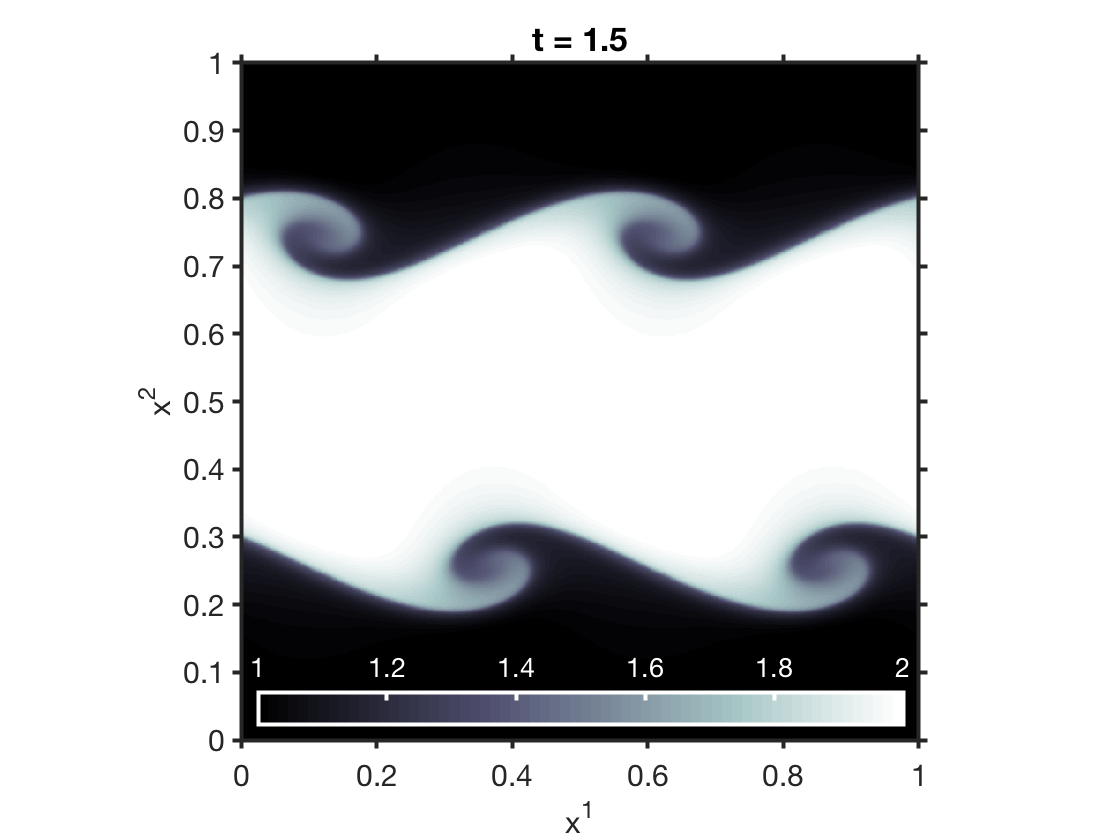
\includegraphics[width=18pc]{./Figures/KelvinHelmholtz_15_Astronum_2018}
  \end{minipage}\hspace{0.5pc}
  \begin{minipage}{18pc}
    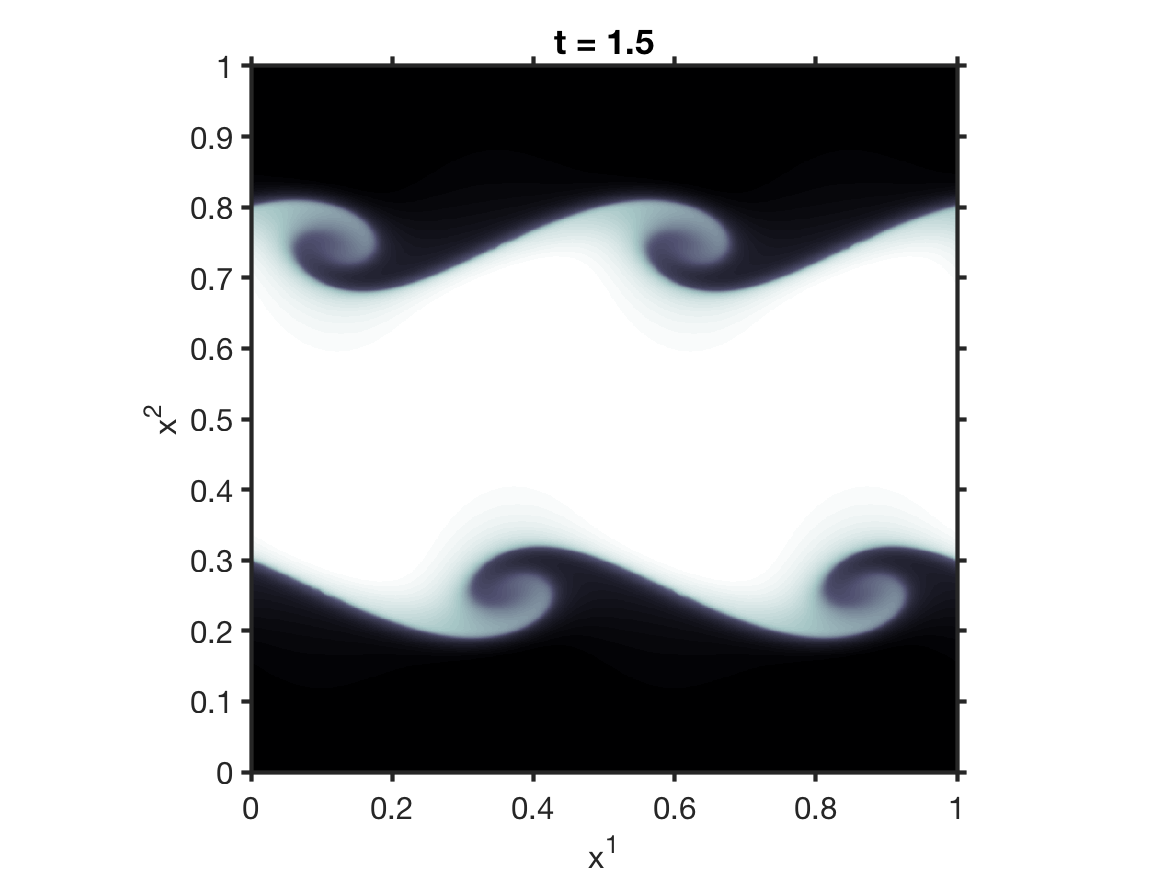
\includegraphics[width=18pc]{./Figures/KelvinHelmholtz_15_noLim_Astronum_2018}
  \end{minipage} \\
  \begin{minipage}{18pc}
    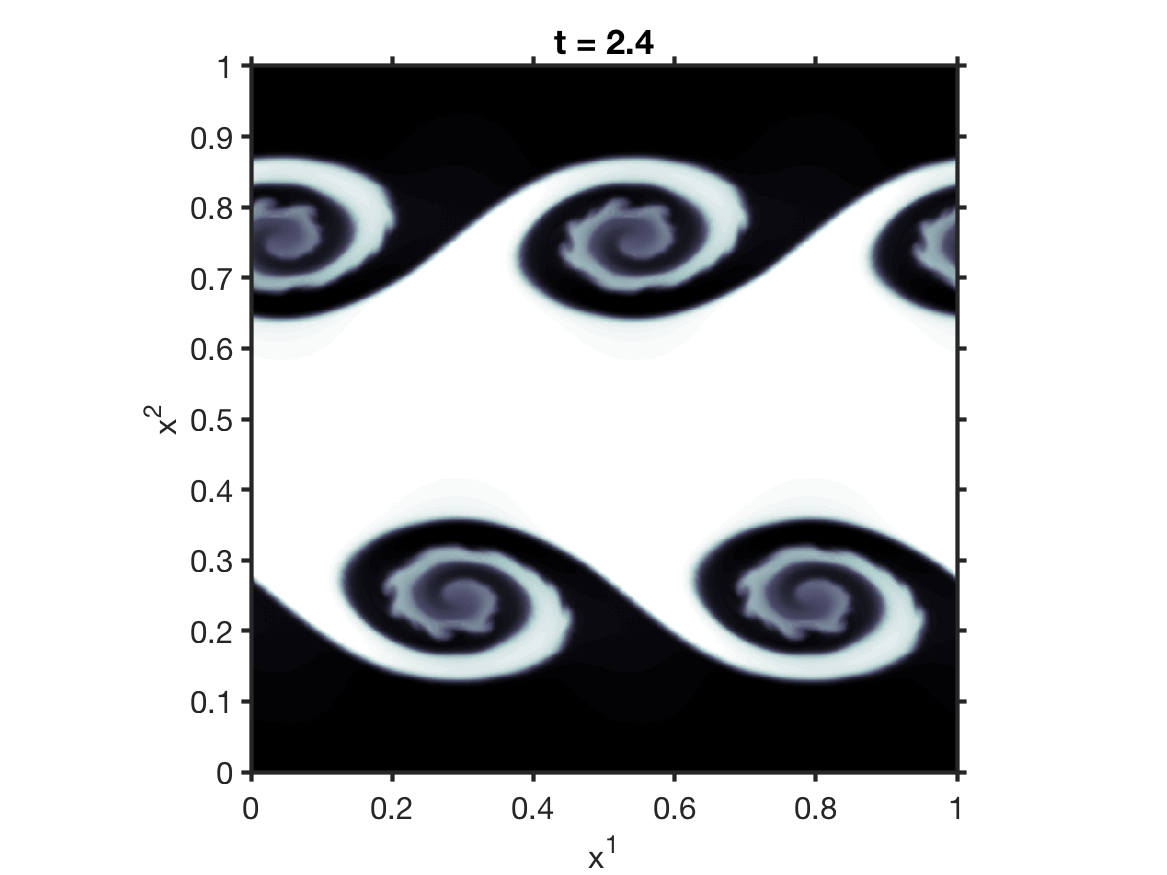
\includegraphics[width=18pc]{./Figures/KelvinHelmholtz_24_Astronum_2018}
  \end{minipage}\hspace{0.5pc}
  \begin{minipage}{18pc}
    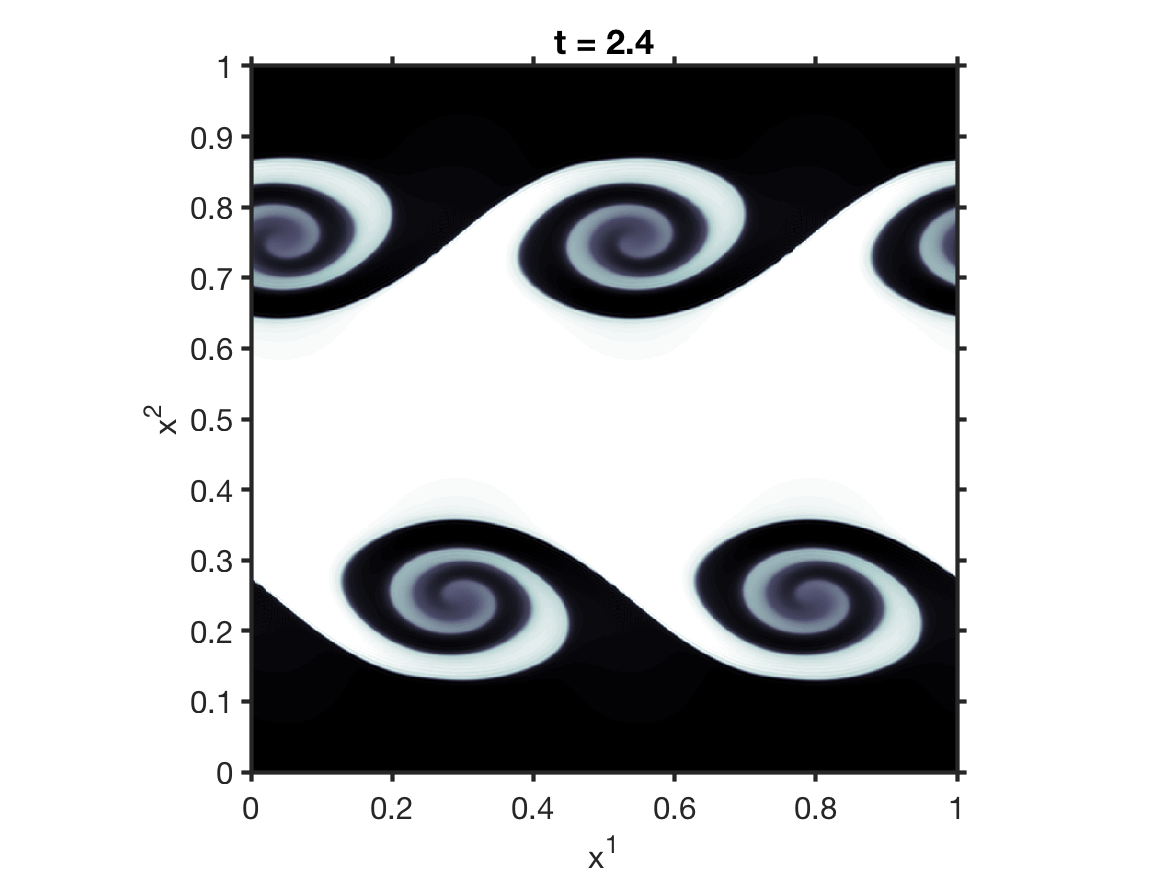
\includegraphics[width=18pc]{./Figures/KelvinHelmholtz_24_noLim_Astronum_2018}
  \end{minipage} \\
  \begin{minipage}{18pc}
    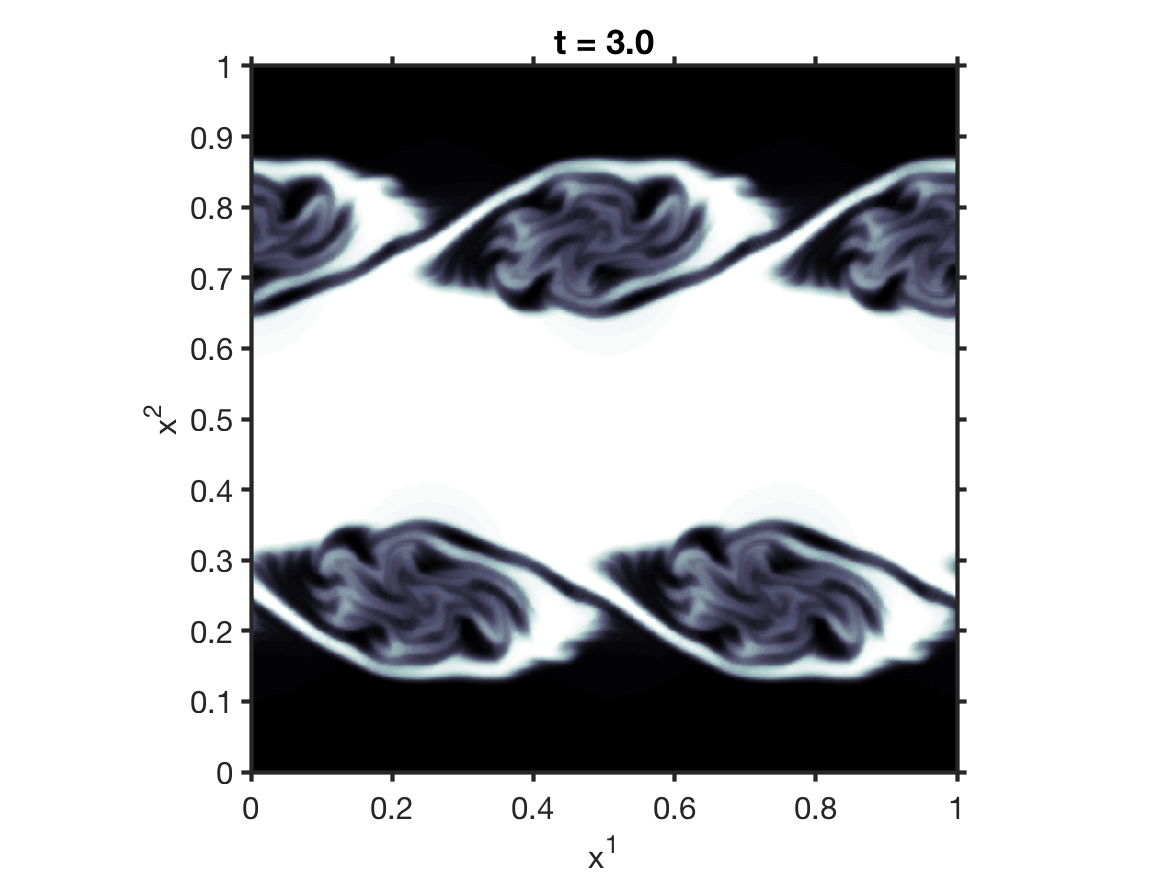
\includegraphics[width=18pc]{./Figures/KelvinHelmholtz_30_Astronum_2018}
  \end{minipage}\hspace{0.5pc}
  \begin{minipage}{18pc}
    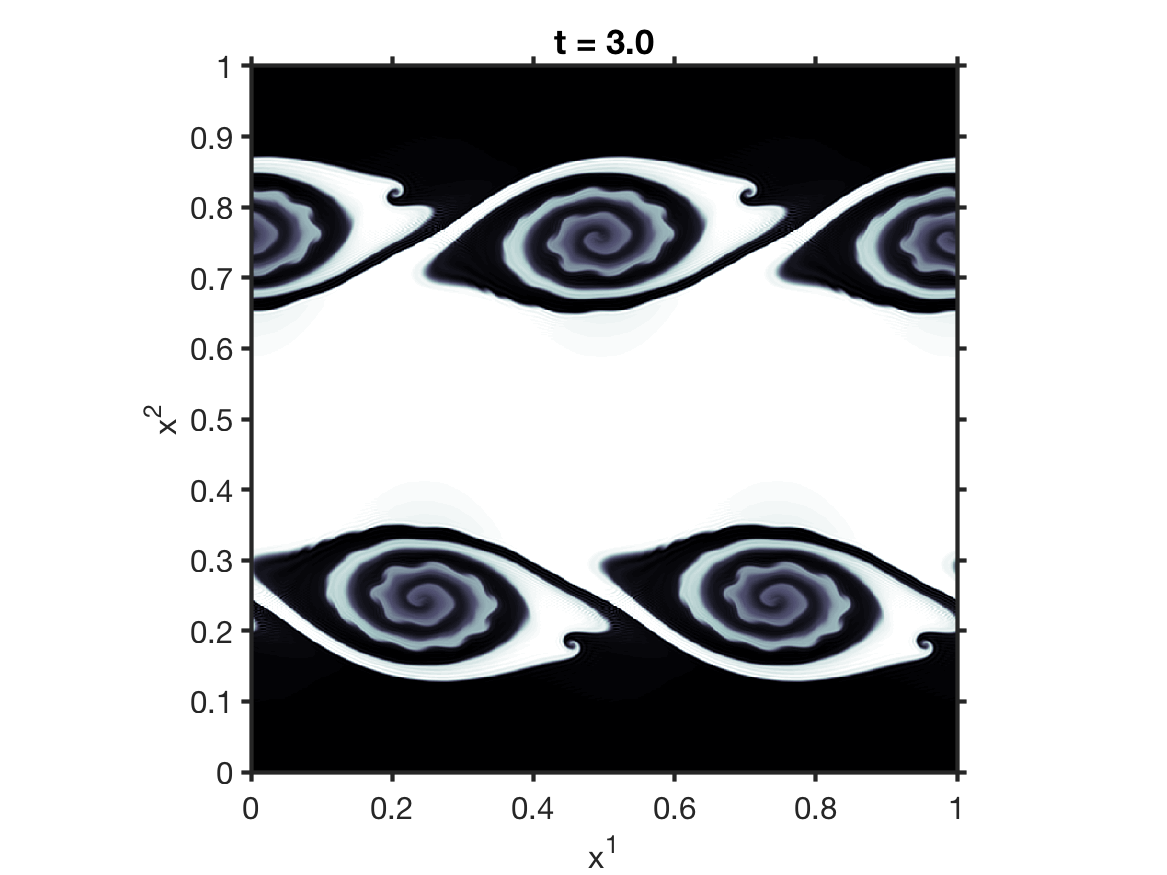
\includegraphics[width=18pc]{./Figures/KelvinHelmholtz_30_noLim_Astronum_2018}
  \end{minipage}
  \caption{\label{fig:KelvinHelmholtz}Mass density from the KH instability at various times, computed with $256^{2}$ elements: $t=1.5$ (top panels), $t=2.4$ (middle panels), and $t=3.0$ (bottom panels).  Results for $C_{\TCI}=0.06$ are shown in left panels, while result with no limiting are shown in right panels.}
\end{figure}

Early on ($t=1.5$), the results from the two runs are practically indistinguishable, show no sign of developing secondary billows, and agree visually with results presented in \cite{mcnally_etal_2012}.  
When $t=2.4$, the run with $C_{\TCI}=0.03$ has started to develop secondary billows within the coiled-up interface separating dense (white) and light (black) fluids, while the model with no limiting has not.  
When $t=3.0$, these secondary instabilities appear to have largely destroyed the coil structure for the model with limiting, while the coils remain intact in the model without limiting (although secondary billows have started to form in this model at this time).  
As discussed in more detail by \cite{mcnally_etal_2012}, the development of the secondary billows may be an artifact of numerical perturbations and diffusion, which is delayed when the resolution is increased.  
Our results are consistent with this in the sense that the less diffusive model develops secondary billows later.  

\subsubsection{Liska-Wendroff Implosion}

This test from \cite{liskaWendroff_2003} is computed on a 2D domain $D=[0,0.3]\times[0,0.3]$ with reflecting boundary conditions using $256^{2}$ elements.  
Below the line $x^{2}=0.15-x^{1}$, we initially set $\vect{U}=\big(0.125,\vect{0.0},0.35\big)^{\trans}$, while $\vect{U}=\big(1.0,\vect{0.0},2.5\big)^{\trans}$ elsewhere.  

\begin{figure}[h]
  \centering
  \begin{minipage}{18pc}
    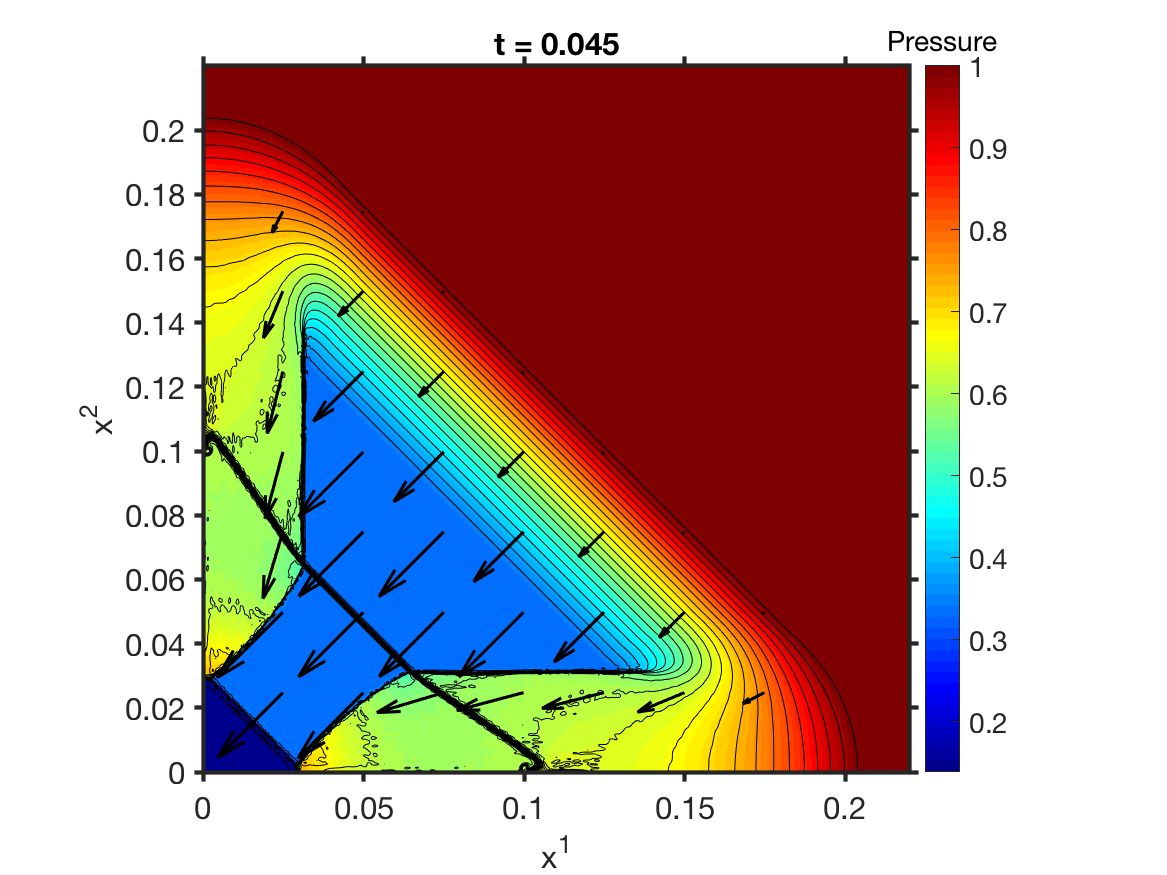
\includegraphics[width=18pc]{./Figures/Implosion_01_HighTCI_Astronum_2018}
  \end{minipage}\hspace{0.5pc}%
  \begin{minipage}{18pc}
    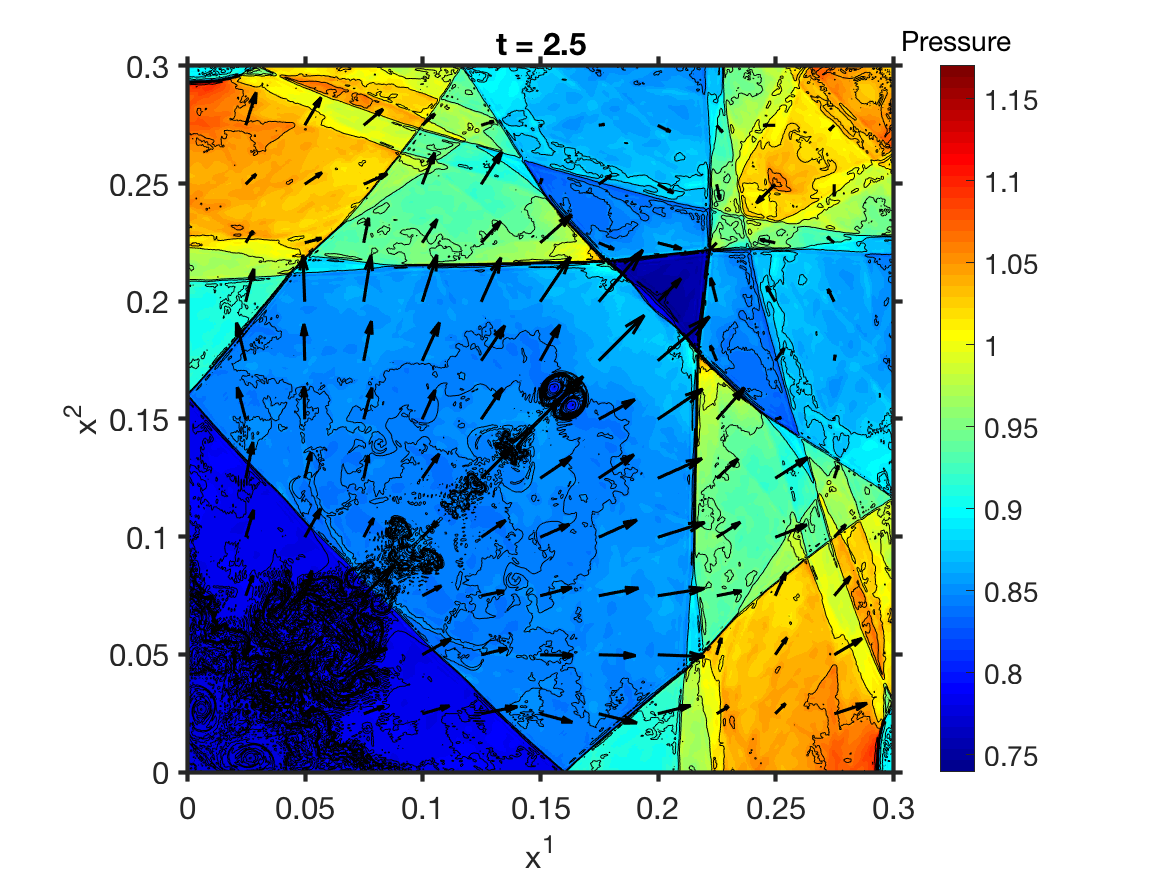
\includegraphics[width=18pc]{./Figures/Implosion_02_HighTCI_Astronum_2018}
  \end{minipage}
  \caption{\label{fig:Implosion}Plots for the Liska-Wendroff implosion problem at $t=0.045$ (left) and $t=2.5$ (right), intended to match Figures~4.10 and 4.11 in \cite{liskaWendroff_2003}.  The color map shows the pressure distribution, black contours show the mass density, while arrows indicate the velocity.}
\end{figure}

Results for $t=0.045$ and $t=2.5$, with $C_{\TCI}=0.6$, are displayed in Figure~\ref{fig:Implosion} (left and right panels, respectively), which agree qualitatively with \cite{liskaWendroff_2003}, who compared the results of eight different schemes for this problem.  
When $t=0.045$, a shock wave propagates towards the origin of $D$, while a contact discontinuity is trailing the shock (cf. density contours), and a rarefaction wave is spreading in the opposite directions.  
When $t=2.5$, a complex flow pattern with multiple shocks has emerged due to multiple reflections off the boundaries.  
The initial symmetry about the $x^{1}=x^{2}$ diagonal is maintained, and the results from \thornado\ agree qualitatively with the unsplit schemes in \cite{liskaWendroff_2003}.  
In the right panel of Figure~\ref{fig:Implosion}, the chatacteristic ``jet'' has formed and propagates along the diagonal, similar to that displayed by CLAW and WENO in \cite{liskaWendroff_2003}.  

\subsubsection{Standing Accretion Shock (SAS)}

This test is of immediate relevance to simulation of CCSNe.  
The initial condition is described in detail in \cite{blondin_etal_2003}, and has been used by many to study the role of the standing accretion shock instability (SASI) on CCSN explosion dynamics.  
We follow closely the description in \cite{blondin_etal_2003} to initialize this test.  
We use spherical polar coordinates, let $D=[0.2,2.0]$, and $\Gamma=4/3$.  
The gravitational potential is given by the point-mass formula with $GM=0.5$.  
A stationary shock is placed at a radius $R_{\shock}=1$.  
Ahead of the shock, the flow is essentially in free-fall towards the shock with a constant Mach number of $100$.  
The mass accretion rate is held fixed at the outer boundary to $\dot{M}=4\pi$.  
Below the shock, $r\in[0.2,1]$, the settling solution is obtained by solving Bernoulli's equation.  
We let matter flow through the inner boundary, and the density and pressure in the boundary elements are set by extrapolating from $D$ assuming $\rho\propto r^{-3}$ and $E\propto r^{-4}$, while the momentum components are held fixed to their initial values.  

\begin{figure}[h]
  \centering
  \begin{minipage}{18pc}
    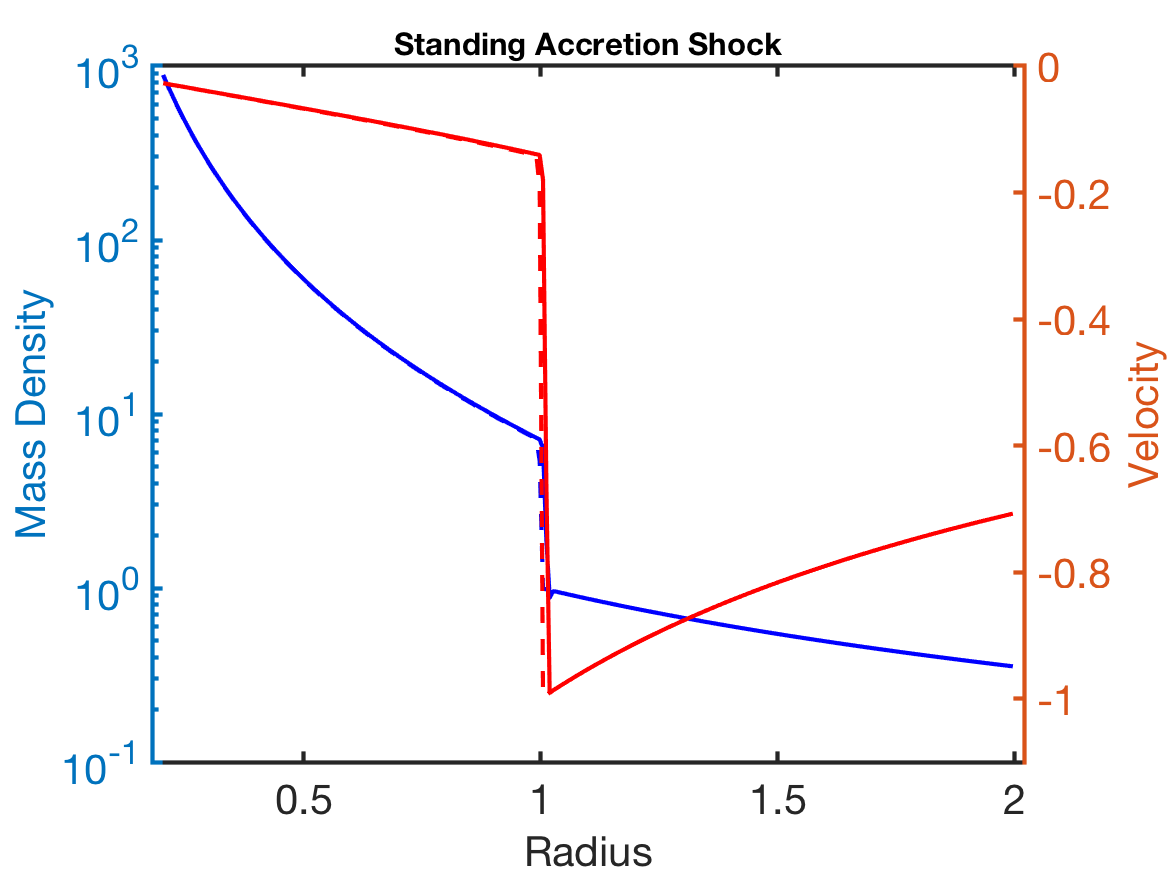
\includegraphics[width=18pc]{./Figures/SAS_Astronum_2018}
  \end{minipage}\hspace{0.5pc}%
  \begin{minipage}{18pc}
    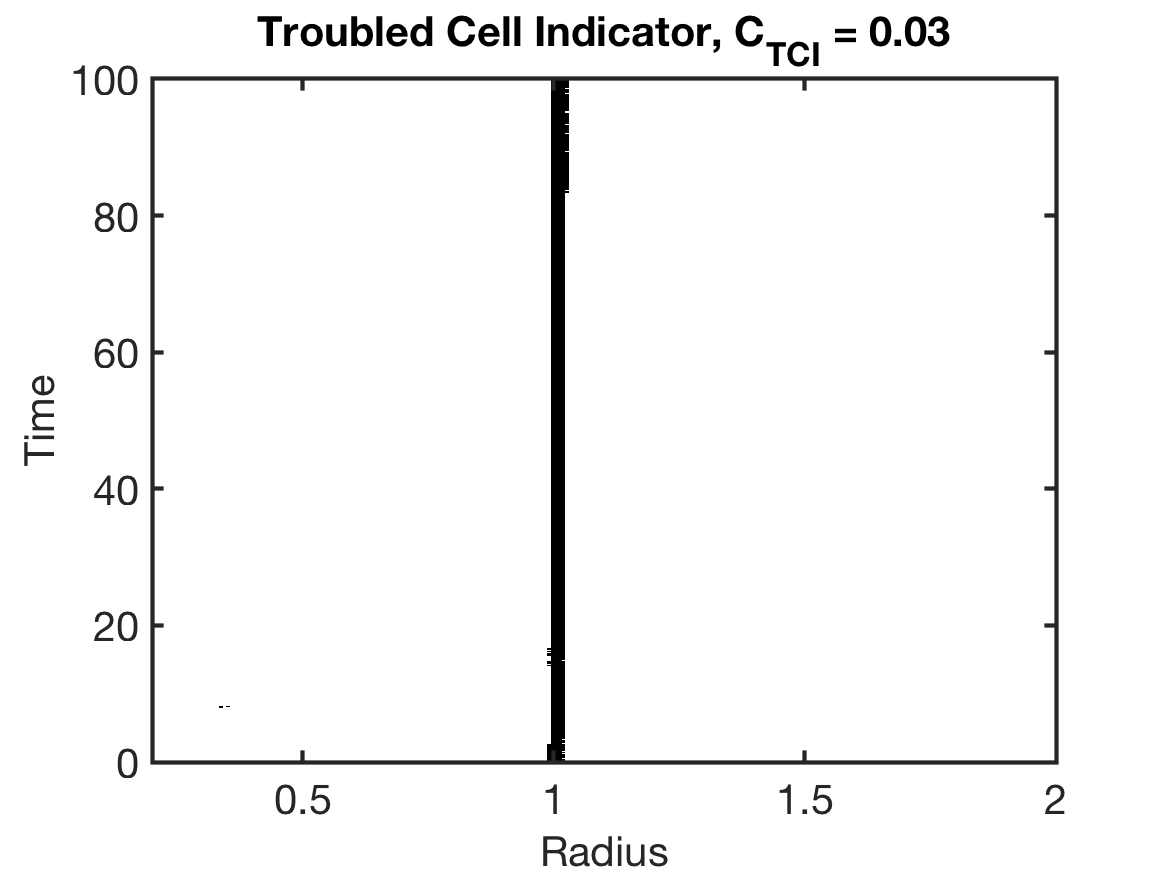
\includegraphics[width=18pc]{./Figures/SAS_TCI_Astronum_2018}
  \end{minipage} \\
  \begin{minipage}{36pc}
    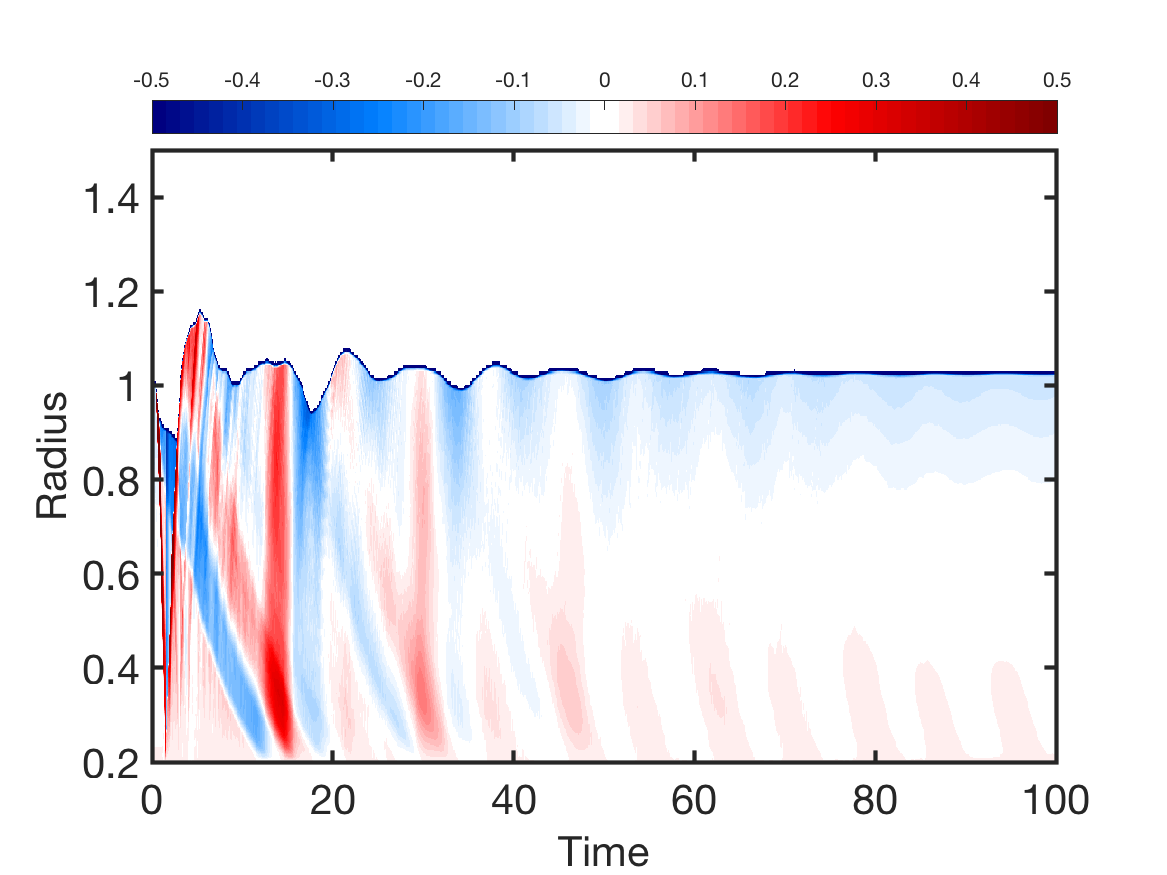
\includegraphics[width=36pc]{./Figures/SAS_Perturbed_Astronum_2018}
  \end{minipage}
  \caption{\label{fig:SAS}Results from the SAS test using $256$ elements.  In the upper left panel we plot the mass density (blue) and velocity (red) versus radius for the initial condition (dashed lines) and for $t=100$ (solid lines) from an unperturbed run.  In the upper right panel we show elements flagged for limiting in the $rt$-plane.  In the bottom panel we show results from a perturbed model, where we plot the relative deviation of the pressure below the shock from; cf. Eq.~\eqref{eq:pressureDeviation}.}
\end{figure}
We use $256$ elements and run the tests until $t=100$ ($>5$ dynamical times \cite{blondin_etal_2003}).  
Results are shown in Figure~\ref{fig:SAS}.  
In the first test we show results from an unperturbed run to gauge the ability of the DG method to maintain the initial state.  
In the upper left panel we compare the initial state (dashed lines) with the solution at $t=100$.  
Except for a slight shift ($\sim1\%$) in the position of the shock, the initial and final states are indistinguishable on the plot.  
Also, there are no oscillations visible in the numerical results.  
In the upper right panel we show elements flagged for limiting in the $rt$-plane (we set $C_{\TCI}=0.03$ in this run), which illustrates how limiting is confined to the shock.  
In the second test we placed a shell ahead of the shock with thickness $0.2$ and density three times higher than the ambient density to induce a strong radial perturbation (similar to \cite{blondin_etal_2003}; see their Figure~4).  
The initial condition we use should be stable against radial perturbations.  
In the lower panel in Figure~\ref{fig:SAS} we plot the pressure deviation below the shock, defined as
\begin{equation}
  \delta p = (p-\bar{p})/\bar{p},
  \quad\text{where}\quad
  \bar{p}=p_{0}(r_{0}/r)^{4},
  \label{eq:pressureDeviation}
\end{equation}
and $p_{0}$ and $r_{0}$ are the pressure and radius closest to the inner boundary.  
As the shell falls through the shock, the perturbation leads to an interesting pattern of waves propagating inside the shocked cavity and oscillations of the shock position, which eventually die out.  
The configuration eventually settles down to something close to the initial condition.  
However, in the final state, the position of the shock is slightly larger than that of the initial state.  

\subsubsection{Yahil-Lattimer Collapse}

The final test of the NR hydrodynamics in \thornado\ involves self-gravity and is due to \cite{yahilLattimer_1982,yahil_1983}.  
It models the self-similar collapse of a polytropic star; i.e., $p=\kappa\rho^{\Gamma}$, where $\kappa$ is the polytropic constant.  
This test is also of immediate relevance to CCSN simulations.  
In \cite{yahilLattimer_1982,yahil_1983}, self-similar solutions to the gravitational collapse problem where constructed for $6/5\le\Gamma<4/3$, which smoothly connect an homologously collapsing subsonic inner core (velocity proportional to radius) to a supersonically collapsing outer core in near free-fall ($u\propto r^{-1/2}$).  
\begin{figure}[h]
  \centering
  \begin{minipage}{18pc}
    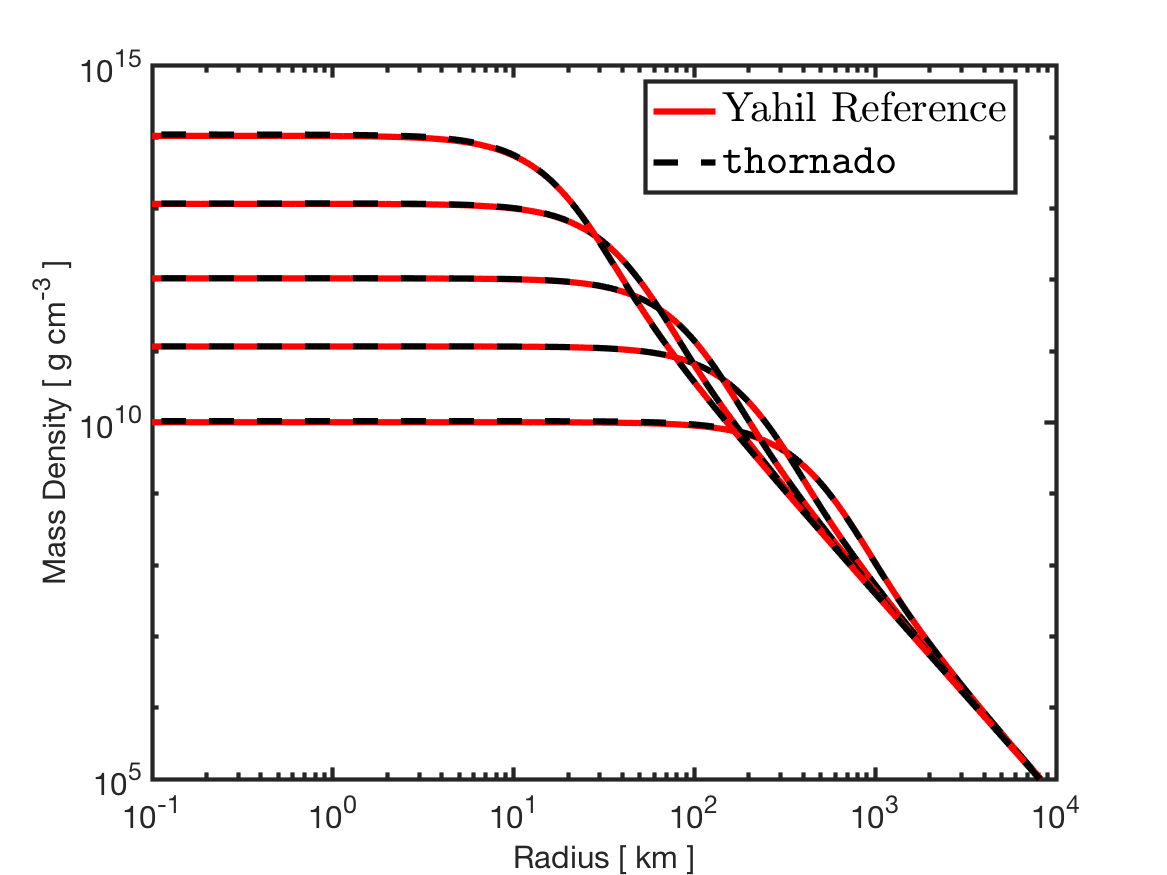
\includegraphics[width=18pc]{./Figures/YahilLattimerCollapse_MassDensity_Astronum_2018}
  \end{minipage}\hspace{0.5pc}%
  \begin{minipage}{18pc}
    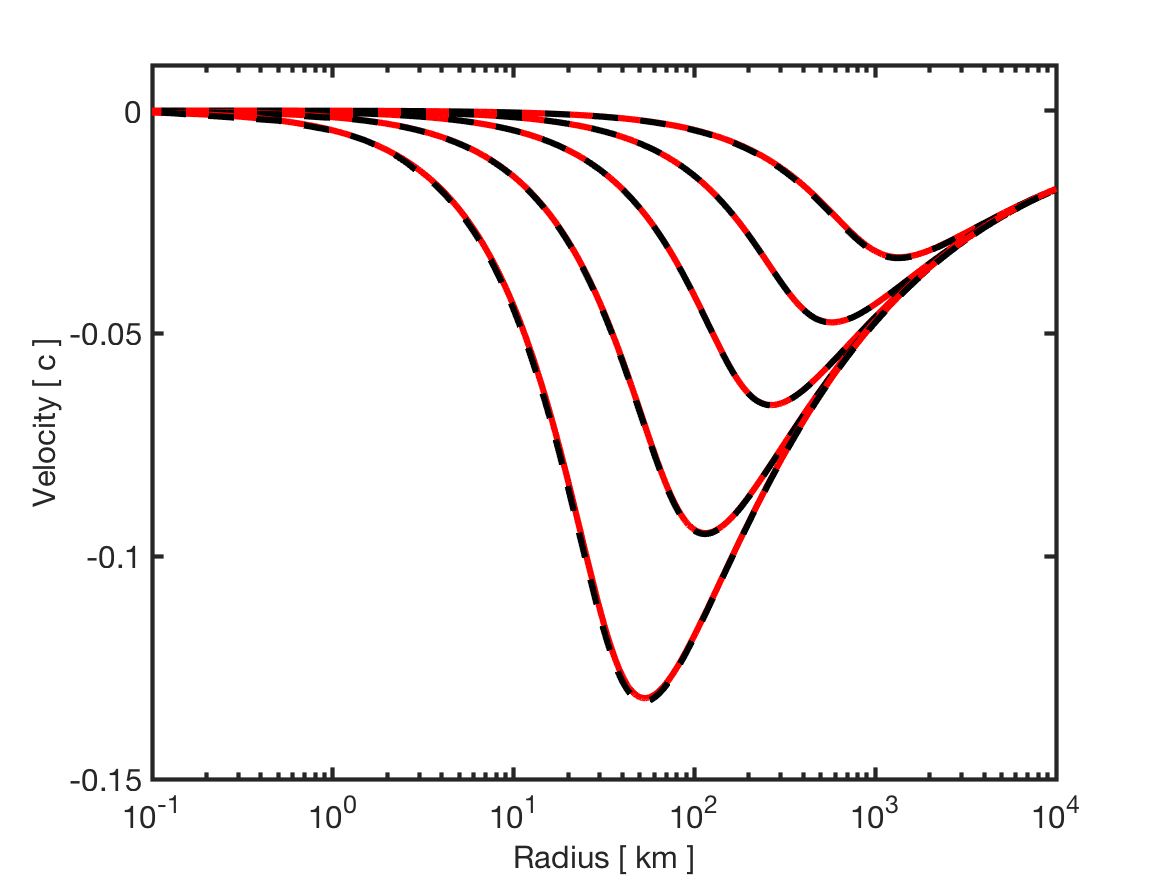
\includegraphics[width=18pc]{./Figures/YahilLattimerCollapse_Velocity_Astronum_2018}
  \end{minipage}
  \caption{\label{fig:YahilLattimer}Results from the Yahil-Lattimer collapse test using $256$ elements.  Results obtained with \thornado\ (dashed black) are compared with the reference solution from Yahil \cite{yahil_1983} (solid red).  The mass density (left panel) and velocity (right panel) are plotted versus radius.  We compare the solutions at select central densities during collapse, approximately $[10^{10},10^{11},10^{12},10^{13},10^{14}]$~g~cm$^{-3}$, which correspond to $(-t)=[51.0,15.0,5.0,1.5,0.5]$~ms.  }
\end{figure}
With two dimensional parameters in the model (the gravitational constant $G$ and the polytropic constant $\kappa$), the dimensionless similarity variable is
\begin{equation}
  X = \kappa^{-1/2} G^{(\Gamma-1)/2} r (-t)^{\Gamma-2},
\end{equation}
where the origin of time is the moment of infinite central density.  
Then all the hydrodynamic variables can be expressed as a function of $X$, and the time-dependent Euler equations can be recast as a system of ODEs (see \cite{yahil_1983} for details).  
To construct a reference to compare with our numerical results we have solved the ODEs given in \cite{yahil_1983} to obtain these self-similar solutions.  

Here we show results for a model with $\Gamma=1.3$.  
We use spherical polar coordinates, and let $D=[0,1\times10^{5}]$~km, which is covered with $256$ elements.  
We use a geometric grid to resolve the mass distribution as the star collapses and the central density increases from about $10^{9}$~g~cm$^{-3}$ to about $10^{14}$~g~cm$^{-3}$.  
The size of the innermost element is set to $1$~km while the last element is about $3\times10^{3}$~km.  
We specify the polytropic constant by setting a reference pressure $p=6\times10^{27}$~erg~cm$^{-3}$ for $\rho=7\times10^{9}$~g~cm$^{-3}$ (reasonable values for a massive star in the pre-collapse stage).  
We also specify the collapse time to $(-t)=150$~ms.  
Results comparing the mass density and velocity of Yahil's reference solution to the solution obtained with \thornado\ using $C_{\TCI}=0.03$ are plotted in Figure~\ref{fig:YahilLattimer}.  
The agreement is good throughout collapse.  

\subsection{Special relativistic (SR) hydrodynamics}

Here we show results from solving the SR Euler equations in Cartesian coordinates with \thornado.
In this case the state, flux, and source vectors in Eq.~\eqref{eq:extendedEulerCompact} are
\begin{equation}
  \vect{U}=\big(\rho W, \rho h W^{2} u_{j},\tau\big)^{\trans},~
  \vect{F}^{i}=\big(\rho W u^{i},\Pi^{i}_{~j},\rho(hW-1)W u^{i}\big)^{\trans},~
  \text{and}~\vect{S}=0,
\end{equation}
where $W$ is the Lorentz factor, $h=1+(e+p)/\rho$ is the specific enthalpy, $\tau=\rho W(hW-1)-p$, and $\Pi^{i}_{~j}=\rho h W^{2} u^{i} u_{j}+p\delta^{i}_{~j}$.  
We solve two Riemann problems and compare the numerical results with exact solutions obtained with the solver from \cite{martiMuller_2003}.  
Let the primitive state vector be $\vect{V}=\big(\rho,\vect{u},p\big)^{\trans}$.  
In the first problem (Riemann problem~1), taken from \cite{mignoneBodo_2005}, we use $\Gamma=4/3$ and
\begin{equation*}
  \vect{V}_{\leftState}=\big(1.0,0.9,0.0,0.0,1.0\big)^{\trans}\quad\text{and}\quad
  \vect{V}_{\rightState}=\big(1.0,0.0,0.0,0.0,10.0\big)^{\trans},
\end{equation*}
while in the second problem (Riemann problem~2), also from \cite{mignoneBodo_2005}, we use $\Gamma=5/3$, and let
\begin{equation*}
  \vect{V}_{\leftState}=\big(1.0,\vect{0.0},10^{3}\big)^{\trans}\quad\text{and}\quad
  \vect{V}_{\rightState}=\big(1.0,\vect{0.0},10^{-2}\big)^{\trans}.  
\end{equation*}
In both problems, the computational domain is $D=[0,1]$, and the discontinuity is initially located at $x^{1}=0.5$, and the solutions are integrated to $t=0.4$.  
Results are plotted in Figure~\ref{fig:RelativisticHydro}.  

\begin{figure}[h]
  \centering
  \begin{minipage}{18pc}
    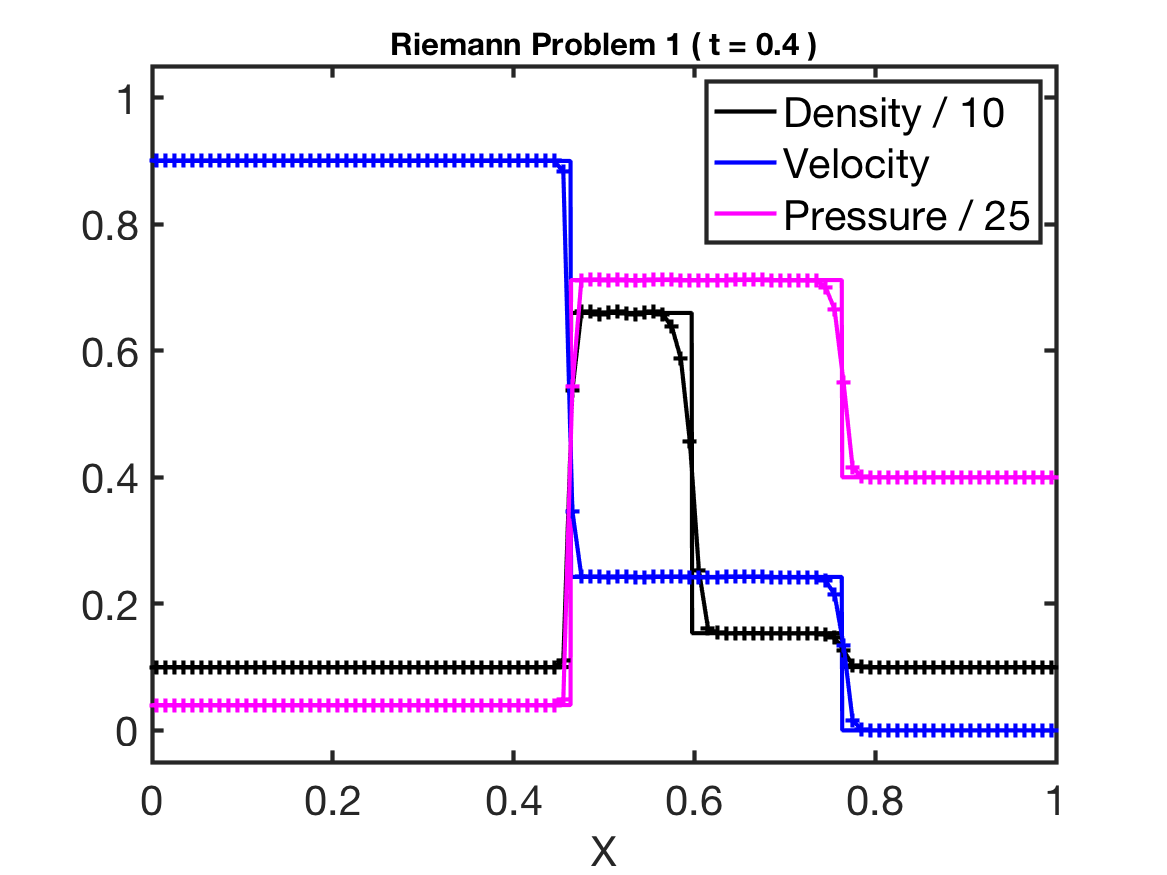
\includegraphics[width=18pc]{./Figures/MB2005_01_Astronum_2018}
  \end{minipage}\hspace{0.5pc}%
  \begin{minipage}{18pc}
    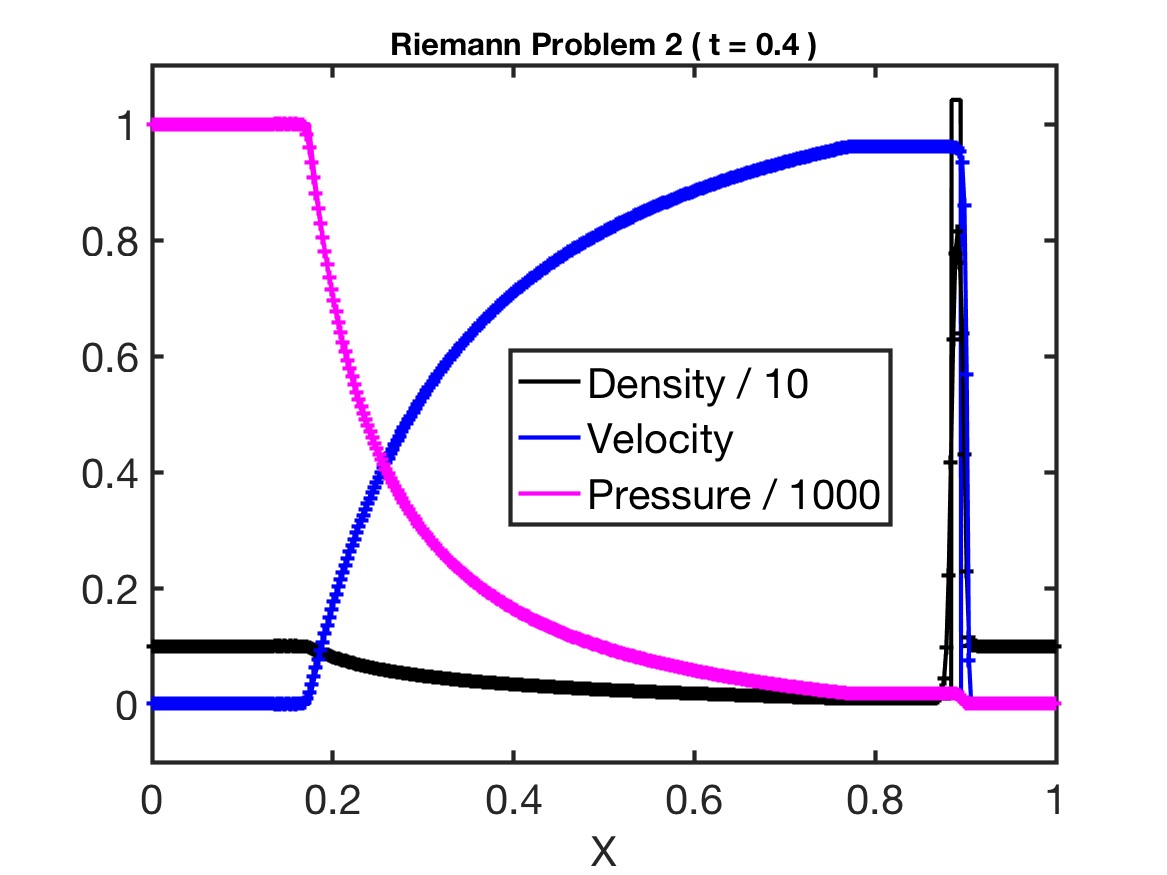
\includegraphics[width=18pc]{./Figures/MB2005_04_Astronum_2018}
  \end{minipage}
  \caption{\label{fig:RelativisticHydro}Results from solving the SR Euler equations with \thornado.  Riemann problem~1 (left panel) was solved using $100$ elements, while Riemann problem~2 was solved using $400$ elements.  The numerical and exact solutions are plotted with plusses and solid lines, respectively.}
\end{figure}

The main features of the exact solution are captured quite well with the DG method implemented in \thornado.  
For Riemann problem~1, there we observe some oscillations in the density between the leftmost shock and the contact discontinuity located near $x^{1}=0.6$.  
For Riemann problem~2, the maximum density in the thin density shell between the shock and the contact discontinuity is significantly lower for the numerical solution than the exact solution.  
This is due to a combination of spatial resolution and the action of the slope limiter.  
We used $C_{\TCI}=0.03$ in both tests in this section.  
We have found the agreement with the exact solution to improve for larger values of $C_{\TCI}$, but at the expense of somewhat more oscillatory results.  

\section{Summary and Outlook}

\ee{Summary and Outlook coming soon.}

We have presented some implementation details and preliminary results of solvers for the Euler equations of gas dynamics in the toolkit for high-order neutrino-radiation hydrodynamics (\thornado).  

The performance of the DG algorithm is sensitive to limiting of the polynomial representation.  

The algorithms in \thornado\ are implemented in Fortran and intended for evolution within logically Cartesian grids.  

Ongoing and future work includes, extension to nuclear equation of state, general relativity within the conformal flatness approximation, porting to hardware accelerators (e.g., GPUs), and deployment within an adaptive mesh refinement framework such as AMREx.  
We hope to report on progress in these directions in the near future.  

\section*{References}
\begin{thebibliography}{24}
  \bibitem{bassi_etal_2013} Bassi, F., Franchina, N. Ghidoni, A., \& Rebay, S. 2013, {\it Int. J. Numer. Meth. Fluids}, {\bf 71}, 1322
  \bibitem{blondin_etal_2003} Blondin, J.M., Mezzacappa, A., \& DeMarino, C. 2003, {\it ApJ}, {\bf 584}, 980
  \bibitem{cockburnShu_1998} Cockburn, B. \& Shu, C.-W. 1998, {\it JCP}, {\bf 141}, 199
  \bibitem{cockburnShu_2001} Cockburn, B. \& Shu, C.-W. 2001, {\it Journal of Scientific Computing}, {\bf 16}, 173
  \bibitem{fuShu_2017} Fu, G. \& Shu, C.-W. 2017, {\it JCP}, {\bf 347}, 305
  \bibitem{harten_etal_1983} Harten, A., Lax, P.D., \& Van Leer, B. 1983, {\it SIAM Review}, {\bf 25}, 35
  \bibitem{hesthavenWarburton_2008} Hesthaven, J.S. \& Warburton T. 2008, {\it Nodal discontinuous Galerkin methods: Algorithms, analysis and applications}, Springer
  \bibitem{landauLifshitz_1979} Landau, L.D. \& Lifshitz, E.M. 1979, {\it Fluid Mechanics}, Pergamon
  \bibitem{liskaWendroff_2003} Liska, R. \& Wendroff, B. 2003, {\it SIAM J. Sci. Comput.}, {\bf 25}, 3
  \bibitem{martiMuller_2003} Mart{\'i}, J.M. \& M{\"u}ller, E. 2003, {\it Living Rev. Relativ.}, {\bf 6}, 7
  \bibitem{mcnally_etal_2012} McNally, C., Lyra, W., \& Passy, J.-C. 2012, {\it ApJS}, {\bf 201}, 18
  \bibitem{mignoneBodo_2005} Mignone, A. \& Bodo, G. 2005, {\it MNRAS}, {\bf 364}, 126
  \bibitem{qin_etal_2016} Qin, T., Shu, C.-W., \& Yang, Y. 2016, {\it JCP}, {\bf 315}, 323
  \bibitem{sedov_1959} Sedov, L.I. 1959, {\it Similarity and Dimensional Methods in Mechanics}, Academic Press
  \bibitem{shuOsher_1988} Shu, C.-W. \& Osher, S. 1988, {\it JCP}, {\bf 77}, 439
  \bibitem{shuOsher_1989} Shu, C.-W. \& Osher, S. 1989, {\it JCP}, {\bf 83}, 32
  \bibitem{shu_2016} Shu, C.-W. 2016, {\it JCP}, {\bf 316}, 598
  \bibitem{sod_1978} Sod, G.A. 1978, {\it JCP}, {\bf 27}, 1
  \bibitem{toro_etal_1994} Toro, E.F., Spruce, M., \& Speares W. 1994, {\it Shock Waves}, {\bf 4}, 25
  \bibitem{toro_1999} Toro, E.F. 1999, NUMERICA: A Library of Source Codes for Teaching, Research and Applications
  \bibitem{wuTang_2015} Wu, K. \& Tang, H. 2015, {\it JCP}, {\bf 298}, 539
  \bibitem{yahilLattimer_1982} Yahil, A. \& Lattimer, J.M. 1982, {\it Supernovae: A Survey of Current Research}, Reidel
  \bibitem{yahil_1983} Yahil, A. 1983, {\it ApJ}, {\bf 265}, 1047
  \bibitem{zhangShu_2010} Zhang, X. \& Shu, C.-W. 2010, {\it JCP}, {\bf 229}, 8918
\end{thebibliography}

\clearpage

\section{Introduction}
These guidelines show how to prepare articles for publication in \jpcs\ using \LaTeX\ so they can be published quickly and accurately. Articles will be refereed by the \corg s but the accepted PDF will be published with no editing, proofreading or changes to layout. It is, therefore, the author's responsibility to ensure that the content and layout are correct.  This document has been prepared using \cls\ so serves as a sample document. The class file and accompanying documentation are available from \verb"http://jpcs.iop.org".

\section{Preparing your paper}
\verb"jpconf" requires \LaTeXe\ and  can be used with other package files such
as those loading the AMS extension fonts 
\verb"msam" and \verb"msbm" (these fonts provide the 
blackboard bold alphabet and various extra maths symbols as well as 
symbols useful in figure captions); an extra style file \verb"iopams.sty" is 
provided to load these packages and provide extra definitions for bold Greek letters. 
\subsection{Headers, footers and page numbers}
Authors should {\it not} add headers, footers or page numbers to the pages of their article---they will
be added by \iopp\ as part of the production process.

\subsection{{\cls\ }package options}
The \cls\ class file has two options `a4paper' and `letterpaper':
\begin{verbatim}
\documentclass[a4paper]{jpconf}
\end{verbatim}

or \begin{verbatim}
\documentclass[letterpaper]{jpconf}
\end{verbatim}

\begin{center}
\begin{table}[h]
\caption{\label{opt}\cls\ class file options.}
%\footnotesize\rm
\centering
\begin{tabular}{@{}*{7}{l}}
\br
Option&Description\\
\mr
\verb"a4paper"&Set the paper size and margins for A4 paper.\\
\verb"letterpaper"&Set the paper size and margins for US letter paper.\\
\br
\end{tabular}
\end{table}
\end{center}

The default paper size is A4 (i.e., the default option is {\tt a4paper}) but this can be changed to Letter by 
using \verb"\documentclass[letterpaper]{jpconf}". It is essential that you do not put macros into the text which alter the page dimensions.

\section{The title, authors, addresses and abstract} 
The code for setting the title page information is slightly different from
the normal default in \LaTeX\ but please follow these instructions as carefully as possible so all articles within a conference have the same style to the title page. 
The title is set in bold unjustified type using the command
\verb"\title{#1}", where \verb"#1" is the title of the article. The
first letter of the title should be capitalized with the rest in lower case. 
The next information required is the list of all authors' names followed by 
the affiliations. For the authors' names type \verb"\author{#1}", 
where \verb"#1" is the 
list of all authors' names. The style for the names is initials then
surname, with a comma after all but the last 
two names, which are separated by `and'. Initials should {\it not} have 
full stops. First names may be used if desired. The command \verb"\maketitle" is not
required.

The addresses of the authors' affiliations follow the list of authors. 
Each address should be set by using
\verb"\address{#1}" with the address as the single parameter in braces. 
If there is more 
than one address then a superscripted number, followed by a space, should come at the start of
each address. In this case each author should also have a superscripted number or numbers following their name to indicate which address is the appropriate one for them.
 
Please also provide e-mail addresses for any or all of the authors using an \verb"\ead{#1}" command after the last address. \verb"\ead{#1}" provides the text Email: so \verb"#1" is just the e-mail address or a list of emails.  

The abstract follows the addresses and
should give readers concise information about the content 
of the article and should not normally exceed 200 
words. {\bf All articles must include an abstract}. To indicate the start 
of the abstract type \verb"\begin{abstract}" followed by the text of the 
abstract.  The abstract should normally be restricted 
to a single paragraph and is terminated by the command
\verb"\end{abstract}"

\subsection{Sample coding for the start of an article}
\label{startsample}
The code for the start of a title page of a typical paper might read:
\begin{verbatim}
\title{The anomalous magnetic moment of the 
neutrino and its relation to the solar neutrino problem}

\author{P J Smith$^1$, T M Collins$^2$, 
R J Jones$^{3,}$\footnote[4]{Present address:
Department of Physics, University of Bristol, Tyndalls Park Road, 
Bristol BS8 1TS, UK.} and Janet Williams$^3$}

\address{$^1$ Mathematics Faculty, Open University, 
Milton Keynes MK7~6AA, UK}
\address{$^2$ Department of Mathematics, 
Imperial College, Prince Consort Road, London SW7~2BZ, UK}
\address{$^3$ Department of Computer Science, 
University College London, Gower Street, London WC1E~6BT, UK}

\ead{williams@ucl.ac.uk}

\begin{abstract}
The abstract appears here.
\end{abstract}
\end{verbatim}

\section{The text}
The text of the article should should be produced using standard \LaTeX\ formatting. Articles may be divided into sections and subsections, but the length limit provided by the \corg\ should be adhered to.

\subsection{Acknowledgments}
Authors wishing to acknowledge assistance or encouragement from 
colleagues, special work by technical staff or financial support from 
organizations should do so in an unnumbered Acknowledgments section 
immediately following the last numbered section of the paper. The 
command \verb"\ack" sets the acknowledgments heading as an unnumbered
section.

\subsection{Appendices}
Technical detail that it is necessary to include, but that interrupts 
the flow of the article, may be consigned to an appendix. 
Any appendices should be included at the end of the main text of the paper, after the acknowledgments section (if any) but before the reference list.
If there are two or more appendices they will be called Appendix A, Appendix B, etc. 
Numbered equations will be in the form (A.1), (A.2), etc,
figures will appear as figure A1, figure B1, etc and tables as table A1,
table B1, etc.

The command \verb"\appendix" is used to signify the start of the
appendixes. Thereafter \verb"\section", \verb"\subsection", etc, will 
give headings appropriate for an appendix. To obtain a simple heading of 
`Appendix' use the code \verb"\section*{Appendix}". If it contains
numbered equations, figures or tables the command \verb"\appendix" should
precede it and \verb"\setcounter{section}{1}" must follow it. 

\section{References}
%%%%%%%%%%%%%%%%%%%%%%%%%%%%%%%%%%%%%%%%%%%
In the online version of \jpcs\ references will be linked to their original source or to the article within a secondary service such as INSPEC or ChemPort wherever possible. To facilitate this linking extra care should be taken when preparing reference lists. 

Two different styles of referencing are in common use: the Harvard alphabetical system and the Vancouver numerical system.  For \jpcs, the Vancouver numerical system is preferred but authors should use the Harvard alphabetical system if they wish to do so. In the numerical system references are numbered sequentially throughout the text within square brackets, like this [2], and one number can be used to designate several references.  

\subsection{Using \BibTeX}
We highly recommend the {\ttfamily\textbf\selectfont iopart-num} \BibTeX\ package by Mark~A~Caprio \cite{iopartnum}, which is included with this documentation.

\subsection{Reference lists}
A complete reference should provide the reader with enough information to locate the article concerned, whether published in print or electronic form, and should, depending on the type of reference, consist of:  

\begin{itemize}
\item name(s) and initials;
\item date published;
\item title of journal, book or other publication; 
\item titles of journal articles may also be included (optional);
\item volume number;
\item editors, if any;
\item town of publication and publisher in parentheses for {\it books};
\item the page numbers.
\end{itemize}

Up to ten authors may be given in a particular reference; where 
there are more than ten only the first should be given followed by 
`{\it et al}'. If an author is unsure of a particular journal's abbreviated title it is best to leave the title in 
full. The terms {\it loc.\ cit.\ }and {\it ibid.\ }should not be used. 
Unpublished conferences and reports should generally not be included 
in the reference list and articles in the course of publication should 
be entered only if the journal of publication is known. 
A thesis submitted for a higher degree may be included 
in the reference list if it has not been superseded by a published 
paper and is available through a library; sufficient information 
should be given for it to be traced readily.

\subsection{Formatting reference lists}
Numeric reference lists should contain the references within an unnumbered section (such as \verb"\section*{References}"). The 
reference list itself is started by the code 
\verb"\begin{thebibliography}{<num>}", where \verb"<num>" is the largest
number in the reference list and is completed by
\verb"\end{thebibliography}". 
Each reference starts with \verb"\bibitem{<label>}", where `label' is the label used for cross-referencing. Each \verb"\bibitem" should only contain a reference to a single article (or a single article and a preprint reference to the same article).  When one number actually covers a group of two or more references to different articles, \verb"\nonum"
should replace \verb"\bibitem{<label>}" at
the start of each reference in the group after the first.

For an alphabetic reference list use \verb"\begin{thereferences}" ... \verb"\end{thereferences}" instead of the
`thebibliography' environment and each reference can be start with just \verb"\item" instead of \verb"\bibitem{label}"
as cross referencing is less useful for alphabetic references.

\subsection {References to printed journal articles}
A normal reference to a journal article contains three changes of font (see table \ref{jfonts}) and is constructed as follows:

\begin{itemize}
\item the authors should be in the form surname (with only the first letter capitalized) followed by the initials with no periods after the initials. Authors should be separated by a comma except for the last two which should be separated by `and' with no comma preceding it;
\item the article title (if given) should be in lower case letters, except for an initial capital, and should follow the date;
\item the journal title is in italic and is abbreviated. If a journal has several parts denoted by different letters the part letter should be inserted after the journal in Roman type, e.g. {\it Phys. Rev.} A;
\item the volume number should be in bold type;
\item both the initial and final page numbers should be given where possible. The final page number should be in the shortest possible form and separated from the initial page number by an en rule `-- ', e.g. 1203--14, i.e. the numbers `12' are not repeated.
\end{itemize}

A typical (numerical) reference list might begin

\medskip
\begin{thebibliography}{9}
\item Strite S and Morkoc H 1992 {\it J. Vac. Sci. Technol.} B {\bf 10} 1237 
\item Jain S C, Willander M, Narayan J and van Overstraeten R 2000 
{\it J. Appl. Phys}. {\bf 87} 965 
\item Nakamura S, Senoh M, Nagahama S, Iwase N, Yamada T, Matsushita T, Kiyoku H 
and 	Sugimoto Y 1996 {\it Japan. J. Appl. Phys.} {\bf 35} L74 
\item Akasaki I, Sota S, Sakai H, Tanaka T, Koike M and Amano H 1996 
{\it Electron. Lett.} {\bf 32} 1105 
\item O'Leary S K, Foutz B E, Shur M S, Bhapkar U V and Eastman L F 1998 
{\it J. Appl. Phys.} {\bf 83} 826 
\item Jenkins D W and Dow J D 1989 {\it Phys. Rev.} B {\bf 39} 3317 
\end{thebibliography}
\smallskip

\noindent which would be obtained by typing

\begin{verbatim}
\begin{\thebibliography}{9}
\item Strite S and Morkoc H 1992 {\it J. Vac. Sci. Technol.} B {\bf 10} 1237 
\item Jain S C, Willander M, Narayan J and van Overstraeten R 2000 
{\it J. Appl. Phys}. {\bf 87} 965 
\item Nakamura S, Senoh M, Nagahama S, Iwase N, Yamada T, Matsushita T, Kiyoku H 
and 	Sugimoto Y 1996 {\it Japan. J. Appl. Phys.} {\bf 35} L74 
\item Akasaki I, Sota S, Sakai H, Tanaka T, Koike M and Amano H 1996 
{\it Electron. Lett.} {\bf 32} 1105 
\item O'Leary S K, Foutz B E, Shur M S, Bhapkar U V and Eastman L F 1998 
{\it J. Appl. Phys.} {\bf 83} 826 
\item Jenkins D W and Dow J D 1989 {\it Phys. Rev.} B {\bf 39} 3317 
\end{\thebibliography}
\end{verbatim}

\begin{center}
\begin{table}[h]
\centering
\caption{\label{jfonts}Font styles for a reference to a journal article.} 
\begin{tabular}{@{}l*{15}{l}}
\br
Element&Style\\
\mr
Authors&Roman type\\
Date&Roman type\\
Article title (optional)&Roman type\\
Journal title&Italic type\\
Volume number&Bold type\\
Page numbers&Roman type\\
\br
\end{tabular}
\end{table}
\end{center}

\subsection{References to \jpcs\ articles}
Each conference proceeding published in \jpcs\ will be a separate {\it volume}; 
references should follow the style for conventional printed journals. For example:\vspace{6pt}
\numrefs{1}
\item Douglas G 2004 \textit{J. Phys.: Conf. Series} \textbf{1} 23--36
\endnumrefs

%%%%%%%%%%%%%%%%%%%%%%%%%%%%%%%%%%
\subsection{References to preprints}
For preprints there are two distinct cases:
\renewcommand{\theenumi}{\arabic{enumi}}
\begin{enumerate}
\item Where the article has been published in a journal and the preprint is supplementary reference information. In this case it should be presented as:
\medskip
\numrefs{1}
\item Kunze K 2003 T-duality and Penrose limits of spatially homogeneous and inhomogeneous cosmologies {\it Phys. Rev.} D {\bf 68} 063517 ({\it Preprint} gr-qc/0303038)
\endnumrefs
\item Where the only reference available is the preprint. In this case it should be presented as
\medskip
\numrefs{1}
\item Milson R, Coley A, Pravda V and Pravdova A 2004 Alignment and algebraically special tensors {\it Preprint} gr-qc/0401010
\endnumrefs
\end{enumerate}

\subsection{References to electronic-only journals}
In general article numbers are given, and no page ranges, as most electronic-only journals start each article on page 1.

\begin{itemize} 
\item For {\it New Journal of Physics} (article number may have from one to three digits)
\numrefs{1}
\item Fischer R 2004 Bayesian group analysis of plasma-enhanced chemical vapour deposition data {\it New. J. Phys.} {\bf 6} 25 
\endnumrefs
\item For SISSA journals the volume is divided into monthly issues and these form part of the article number

\numrefs{2}
\item Horowitz G T and Maldacena J 2004 The black hole final state {\it J. High Energy Phys.}  	JHEP02(2004)008
\item Bentivegna E, Bonanno A and Reuter M 2004 Confronting the IR fixed point cosmology 	with 	high-redshift observations {\it J. Cosmol. Astropart. Phys.} JCAP01(2004)001  
\endnumrefs
\end{itemize} 

\subsection{References to books, conference proceedings and reports}
References to books, proceedings and reports are similar to journal references, but have 
only two changes of font (see table~\ref{book}). 

\begin{table}
\centering
\caption{\label{book}Font styles for references to books, conference proceedings and reports.}
\begin{tabular}{@{}l*{15}{l}}
\br
Element&Style\\
\mr
Authors&Roman type\\
Date&Roman type\\
Book title (optional)&Italic type\\
Editors&Roman type\\
Place (city, town etc) of publication&Roman type\\
Publisher&Roman type\\
Volume&Roman type\\
Page numbers&Roman type\\
\br
\end{tabular}
\end{table}

Points to note are:
\medskip
\begin{itemize}
\item Book titles are in italic and should be spelt out in full with initial capital letters for all except minor words. Words such as Proceedings, Symposium, International, Conference, Second, etc should be abbreviated to {\it Proc.}, {\it Symp.}, {\it Int.}, {\it Conf.}, {\it 2nd}, respectively, but the rest of the title should be given in full, followed by the date of the conference and the town or city where the conference was held. For Laboratory Reports the Laboratory should be spelt out wherever possible, e.g. {\it Argonne National Laboratory Report}.
\item The volume number, for example vol 2, should be followed by the editors, if any, in a form such as `ed A J Smith and P R Jones'. Use {\it et al} if there are more than two editors. Next comes the town of publication and publisher, within brackets and separated by a colon, and finally the page numbers preceded by p if only one number is given or pp if both the initial and final numbers are given.
\end{itemize}

Examples taken from published papers:
\medskip

\numrefs{99}
\item Kurata M 1982 {\it Numerical Analysis for Semiconductor Devices} (Lexington, MA: Heath)
\item Selberherr S 1984 {\it Analysis and Simulation of Semiconductor Devices} (Berlin: Springer)
\item Sze S M 1969 {\it Physics of Semiconductor Devices} (New York: Wiley-Interscience)
\item Dorman L I 1975 {\it Variations of Galactic Cosmic Rays} (Moscow: Moscow State University Press) p 103
\item Caplar R and Kulisic P 1973 {\it Proc. Int. Conf. on Nuclear Physics (Munich)} vol 1 (Amsterdam: 	North-Holland/American Elsevier) p 517
\item Cheng G X 2001 {\it Raman and Brillouin Scattering-Principles and Applications} (Beijing: Scientific) 
\item Szytula A and Leciejewicz J 1989 {\it Handbook on the Physics and Chemistry of Rare Earths} vol 12, ed K A Gschneidner Jr and L Erwin (Amsterdam: Elsevier) p 133
\item Kuhn T 1998 {\it Density matrix theory of coherent ultrafast dynamics Theory of Transport Properties of Semiconductor Nanostructures} (Electronic Materials vol 4) ed E Sch\"oll (London: Chapman and Hall) chapter 6 pp 173--214
\endnumrefs

\section{Tables and table captions}
Tables should be numbered serially and referred to in the text 
by number (table 1, etc, {\bf rather than} tab. 1). Each table should be a float and be positioned within the text at the most convenient place near to where it is first mentioned in the text. It should have an 
explanatory caption which should be as concise as possible. 

\subsection{The basic table format}
The standard form for a table is:
\begin{verbatim}
\begin{table}
\caption{\label{label}Table caption.}
\begin{center}
\begin{tabular}{llll}
\br
Head 1&Head 2&Head 3&Head 4\\
\mr
1.1&1.2&1.3&1.4\\
2.1&2.2&2.3&2.4\\
\br
\end{tabular}
\end{center}
\end{table}
\end{verbatim}

The above code produces table~\ref{ex}.

\begin{table}[h]
\caption{\label{ex}Table caption.}
\begin{center}
\begin{tabular}{llll}
\br
Head 1&Head 2&Head 3&Head 4\\
\mr
1.1&1.2&1.3&1.4\\
2.1&2.2&2.3&2.4\\
\br
\end{tabular}
\end{center}
\end{table}

Points to note are:
\medskip
\begin{enumerate}
\item The caption comes before the table.
\item The normal style is for tables to be centred in the same way as
equations. This is accomplished
by using \verb"\begin{center}" \dots\ \verb"\end{center}".

\item The default alignment of columns should be aligned left.

\item Tables should have only horizontal rules and no vertical ones. The rules at
the top and bottom are thicker than internal rules and are set with
\verb"\br" (bold rule). 
The rule separating the headings from the entries is set with
\verb"\mr" (medium rule). These commands do not need a following double backslash.

\item Numbers in columns should be aligned as appropriate, usually on the decimal point;
to help do this a control sequence \verb"\lineup" has been defined 
which sets \verb"\0" equal to a space the size of a digit, \verb"\m"
to be a space the width of a minus sign, and \verb"\-" to be a left
overlapping minus sign. \verb"\-" is for use in text mode while the other
two commands may be used in maths or text.
(\verb"\lineup" should only be used within a table
environment after the caption so that \verb"\-" has its normal meaning
elsewhere.) See table~\ref{tabone} for an example of a table where
\verb"\lineup" has been used.
\end{enumerate}

\begin{table}[h]
\caption{\label{tabone}A simple example produced using the standard table commands 
and $\backslash${\tt lineup} to assist in aligning columns on the 
decimal point. The width of the 
table and rules is set automatically by the 
preamble.} 

\begin{center}
\lineup
\begin{tabular}{*{7}{l}}
\br                              
$\0\0A$&$B$&$C$&\m$D$&\m$E$&$F$&$\0G$\cr 
\mr
\0\023.5&60  &0.53&$-20.2$&$-0.22$ &\01.7&\014.5\cr
\0\039.7&\-60&0.74&$-51.9$&$-0.208$&47.2 &146\cr 
\0123.7 &\00 &0.75&$-57.2$&\m---   &---  &---\cr 
3241.56 &60  &0.60&$-48.1$&$-0.29$ &41   &\015\cr 
\br
\end{tabular}
\end{center}
\end{table}
 
\section{Figures and figure captions}
Figures must be included in the source code of an article at the appropriate place in the text not grouped together at the end. 

Each figure should have a brief caption describing it and, if 
necessary, interpreting the various lines and symbols on the figure. 
As much lettering as possible should be removed from the figure itself and 
included in the caption. If a figure has parts, these should be 
labelled ($a$), ($b$), ($c$), etc. 
\Tref{blobs} gives the definitions for describing symbols and lines often
used within figure captions (more symbols are available
when using the optional packages loading the AMS extension fonts).

\begin{table}[h]
\caption{\label{blobs}Control sequences to describe lines and symbols in figure 
captions.}
\begin{center}
\begin{tabular}{lllll}
\br
Control sequence&Output&&Control sequence&Output\\
\mr
\verb"\dotted"&\dotted        &&\verb"\opencircle"&\opencircle\\
\verb"\dashed"&\dashed        &&\verb"\opentriangle"&\opentriangle\\
\verb"\broken"&\broken&&\verb"\opentriangledown"&\opentriangledown\\
\verb"\longbroken"&\longbroken&&\verb"\fullsquare"&\fullsquare\\
\verb"\chain"&\chain          &&\verb"\opensquare"&\opensquare\\
\verb"\dashddot"&\dashddot    &&\verb"\fullcircle"&\fullcircle\\
\verb"\full"&\full            &&\verb"\opendiamond"&\opendiamond\\
\br
\end{tabular}
\end{center}
\end{table}


Authors should try and use the space allocated to them as economically as possible. At times it may be convenient to put two figures side by side or the caption at the side of a figure. To put figures side by side, within a figure environment, put each figure and its caption into a minipage with an appropriate width (e.g. 3in or 18pc if the figures are of equal size) and then separate the figures slightly by adding some horizontal space between the two minipages (e.g. \verb"\hspace{.2in}" or \verb"\hspace{1.5pc}". To get the caption at the side of the figure add the small horizontal space after the \verb"\includegraphics" command and then put the \verb"\caption" within a minipage of the appropriate width aligned bottom, i.e. \verb"\begin{minipage}[b]{3in}" etc (see code in this file used to generate figures 1--3).

Note that it may be necessary to adjust the size of the figures (using optional arguments to \verb"\includegraphics", for instance \verb"[width=3in]") to get you article to fit within your page allowance or to obtain good page breaks.

\begin{figure}[h]
\begin{minipage}{14pc}
\includegraphics[width=14pc]{name.eps}
\caption{\label{label}Figure caption for first of two sided figures.}
\end{minipage}\hspace{2pc}%
\begin{minipage}{14pc}
\includegraphics[width=14pc]{name.eps}
\caption{\label{label}Figure caption for second of two sided figures.}
\end{minipage} 
\end{figure}

\begin{figure}[h]
\includegraphics[width=14pc]{name.eps}\hspace{2pc}%
\begin{minipage}[b]{14pc}\caption{\label{label}Figure caption for a narrow figure where the caption is put at the side of the figure.}
\end{minipage}
\end{figure}

Using the graphicx package figures can be included using code such as:
\begin{verbatim}
\begin{figure}
\begin{center}
\includegraphics{file.eps}
\end{center}
\caption{\label{label}Figure caption}
\end{figure}
\end{verbatim}

\section*{References}
\begin{thebibliography}{9}
\bibitem{iopartnum} IOP Publishing is to grateful Mark A Caprio, Center for Theoretical Physics, Yale University, for permission to include the {\tt iopart-num} \BibTeX package (version 2.0, December 21, 2006) with  this documentation. Updates and new releases of {\tt iopart-num} can be found on \verb"www.ctan.org" (CTAN). 
\end{thebibliography}

\end{document}


